% !TeX spellcheck = cs_CZ
%{\tikzset{external/prefix={tikz/FYZI/}}
% \tikzset{external/figure name/.add={ch11_}{}}
%---------------------------------------------------------------------------------------------------
% file fey1ch13_14.tex
%---------------------------------------------------------------------------------------------------
%================ Kapitola: Práce a potenciální energie ============================================
\setchaptertoc
\chapter{Práce a potenciální energie}\label{fyz:chap_fey_work}

  \section{Energie padajícího tělesa}
    V kapitole \ref{fyz:IchapII} jsme se zabývali zachováním energie. Přitom jsme nepoužili 
    Newtonovy zákony, přestože je velmi zajímavé pozorovat, jak se energie podle těchto zákonů 
    zachovává. Pro přehlednost začneme s nejjednodušším možným příkladem a postupně přejdeme k 
    složitějším příkladům.
    
    Nejjednodušším příkladem zachování energie je \emph{těleso padající svisle dolů}, pohybující se 
    ve vertikálním směru. Těleso, jež mění svoji výšku jen na základě gravitace, má při svém pohybu 
    během pádu kinetickou energii \(T\) (nebo \(W_k\)) a potenciální energii \(mgh\), označenou 
    \(U\) (nebo \(W_p\)), jejichž součet se nemění:
    \begin{equation}\label{fyz:eq025}
      \frac{1}{2}mv^2 + mgh = \text{konst,}
    \end{equation}
    \begin{equation*}
      W_k + W_p = \text{konst} \quad \text{nebo} \quad T + U = \text{konst}.
    \end{equation*}
    Nyní bychom chtěli dokázat, že toto tvrzení je správné. Co tím myslíme, že dokážeme správnost? 
    Z druhého Newtonova zákona lze snadno určit pohyb tělesa a zjistit, jak se mění jeho rychlost v 
    závislostí na čase, tj. že roste úměrně s časem a výška tělesa se mění s druhou mocninou času. 
    Když tedy měříme výšku od bodu, kde bylo těleso v klidu, není nic zvláštního na tom, že výška 
    je rovna druhé mocnině času vynásobené několika konstantami. Ale podívejme se na to trochu 
    blíže.
    
    Derivováním kinetické energie podle času a použitím Newtonových zákonů vypočítáme přímo z 
    druhého Newtonova zákona, jak by se měla měnit kinetická energie. Derivováním 
    \(\frac{1}{2}mv^2\) podle času dostáváme
    \begin{equation}\label{fyz:eq026}
      \der{T}{t} = \der{ }{t}\left(\frac{1}{2}mv^2\right) = \frac{1}{2}m2v\der{v}{t} 
                 = mv\der{v}{t},
    \end{equation}
    neboť \(m\) považujeme za konstantu. Z druhého Newtonova zákona vyplývá, že \(m\der{v}{t} = 
    F\), takže
    \begin{equation}\label{fyz:eq027}
      \der{T}{t} =Fv
    \end{equation}
    Obecně dostáváme \(\vec{F}\cdot\vec{v}\), ale v našem jednorozměrném případě můžeme ponechat 
    součin velikosti síly a rychlosti. 
    
    V tomto našem jednoduchém příkladě je síla konstantní, je rovna \(- mg\), má vertikální směr 
    (znaménko minus znamená, že působí směrem dolů) a rychlost je samozřejmě dána změnou vertikální 
    polohy nebo výšky \(h\) s časem. To znamená, že míra změny kinetické energie je \(- 
    mg\der{h}{t}\), což není kupodivu nic jiného, než rychlost změny veličiny \(mgh\). Proto s 
    rostoucím časem jsou si změna kinetické energie a změna veličiny \(mgh\) rovny, až na znaménko, 
    takže součet obou veličin zůstává konstantní.

    \luagraphic[1]{fyz_fig023.pdf}{Těleso pohybující se bez tření po zakřivené trajektorii pod
    vlivem gravitační síly (\cite[s.~186]{Feynman01})}{fyz:fig023}
    
    Na základě druhého Newtonova zákona jsme ukázali, že pro konstantní síly se energie zachovává, 
    jestliže ke kinetické energii \(\frac{1}{2}mv^2\) přičteme potenciální energii \(mgh\). 
    Zkoumejme dále tento poznatek, zda ho lze zobecnit a zda může dále prohloubit naše chápání. 
    Platí jen pro volně padající těleso nebo i obecně? Na základě naší diskuze o zachování energie 
    očekáváme, že by měl platit pro libovolné těleso, jež se pod vlivem gravitace pohybuje bez 
    tření po trajektorii z jednoho bodu do druhého (obr. \ref{fyz:fig023}). Dostane-li se těleso z 
    původní výšky \(H\) do výšky \(h\), měl by znovu platit stejný vztah, ačkoli nyní není směr 
    rychlosti vertikální. Rádi bychom věděli, proč zákon zachování energie ještě platí.
    
    Proveďme stejnou analýzu. Najděme změnu kinetické energie v závislosti na čase. Opět bude    
    rovna \(mv\der{v}{t}\), ale \(m\der{v}{t}\) je rovno \textbf{změně hybnosti}, tj. \emph{síle ve 
    směru pohybu} - tečné síle \(F_t\). Tedy
    \begin{equation}\label{fyz:eq028}
      \der{T}{t} = mv\der{v}{t} = F_tv.
    \end{equation}
    Velikost rychlosti je tedy dána změnou vzdálenosti podél křivky, \(\der{s}{t}\) a tečná síla 
    \(F_t\) není rovna \(mg\), ale je slabší v poměru vzdálenosti \(ds\) podél křivky k vertikální 
    vzdálenosti \(dh\). To znamená
    \begin{align}
      F_t &= -mg\sin\vartheta = -mg\der{h}{s},  \nonumber \\
      \shortintertext{tedy}
      F_t\der{s}{t} = mg\der{h}{s}\der{s}{t}.   \label{fyz:eq029}
    \end{align}
    neboť \(ds\) se vykrátí. Tak, jako v předchozím případě, i nyní jsme dostali veličinu \(- 
    mg\der{h}{t}\), jež je rovna změně \(mgh\).
    
    Aby bylo zcela jasné, jak se zákon zachování energie uplatňuje v mechanice obecně, uvedeme    
    několik pojmů, jež nám pomohou při jeho analýze.
    
    Nejdříve se budeme zabývat změnou kinetické energie v obecném trojrozměrném případě.
    
    V případě pohybu v trojrozměrném prostoru je kinetická energie
    \begin{equation}\label{fyz:eq030}
      T = \frac{1}{2}m(v_x^2 + v_y^2 + v_z^2) \quad\quad 
      T = \frac{1}{2}m\vec{v}\cdot\vec{v}.
    \end{equation}
    Derivováním podle času dostaneme tři hrozivě vypadající členy
    \begin{equation}\label{fyz:eq031}
      \der{T}{t} = m(v_x\der{v_x}{t} + v_y\der{v_y}{t} + v_z\der{v_z}{t}).
    \end{equation}
    Ale \(m\der{v_x}{t}\) je složka síly \(F_x\), jež působí na těleso ve směru osy \(x\), takže 
    pravá strana rovnice \ref{fyz:eq031} je rovna \(F_xv_x + F_yv_y + F_zv_z\) . Podle 
    \emph{vektorové analýzy} je to rovno \(\vec{F}\cdot\vec{v}\), a proto
    \begin{equation}\label{fyz:eq032}
      \der{T}{t} = \vec{F}\cdot\vec{v}.
    \end{equation}
    Tento výsledek lze rychleji odvodit takto: jesdiže \(\vec{a}\) a \(\vec{b}\) jsou dva vektory, 
    které mohou záviset na čase, pak derivace \(\vec{a}\cdot\vec{b}\) je rovna
    \begin{equation}\label{fyz:eq033}
      \der{\vec{a}\cdot\vec{b}}{t} = \vec{a}\cdot\der{\vec{a}}{t} + \vec{b}\cdot\der{\vec{b}}{t}.
    \end{equation}
    Použijeme-li tento vztah pro \(\vec{a}=\vec{b}=\vec{v}\), dostaneme
    \begin{equation}\label{fyz:eq034}
      \der{\left(\frac{1}{2}mv^2\right)}{t} = 
      \der{\left(\frac{1}{2}m\vec{v}\cdot\vec{v}\right)}{t} = 
      m\der{\vec{v}}{t}\cdot\vec{v} = 
      \vec{F}\cdot\vec{v} = 
      \vec{F}\der{\vec{s}}{t}.
    \end{equation}
    Protože pojem kinetické energie a energie vůbec je tak důležitý, dostaly důležité členy v 
    těchto rovnicích své názvy. Jak víme, \(\frac{1}{2}mv^2\) se nazývá \emph{kinetická energie}, 
    \(\vec{F}\cdot\vec{v}\) je \emph{výkon}, síla působící na těleso vynásobená rychlostí tělesa 
    (skalární součin) je výkon dodaný tělesu silou. Takže máme velkolepou větu: \textbf{rychlost 
    změny kinetické energie tělesa je rovna výkonu vynaloženému silami působícími na těleso}.
    
    Abychom dobře prostudovali zákon zachování energie, musíme jít s analýzou ještě dál. Určíme 
    změnu kinetické energie za velmi krátkou dobu \(\dd{t}\)! Vynásobíme-li obě strany rovnice 
    (\ref{fyz:eq034}) \(\dd{t}\), zjistíme, že \emph{diferenciální změna} kinetické energie je 
    rovna skalárnímu součinu síly a diferenciálu dráhy
    \begin{align}
      \dd{T}    &= \vec{F}\cdot\dd{\vec{s}}              \label{fyz:eq035} \\
      \shortintertext{Jestliže tento výraz integrujeme, dostaneme}
      \Delta T  &= \int_{1}^{2}\vec{F}\cdot\dd{\vec{s}}  \label{fyz:eq036}
    \end{align}
    Co to znamená? Znamená to, že pohybuje-li se těleso pod vlivem síly libovolně z jednoho bodu do 
    druhého, je změna kinetické energie rovna integrálu složky síly podél dráhy, vynásobené 
    diferenciálem posunutí \(\dd{s}\), přičemž se integruje od prvního bodu k druhému. Tento 
    integrál má svůj název; je to \textbf{práce vykonaná silou působící na těleso}. Z toho je hned 
    zřejmé, že \textbf{výkon je roven práci vykonané za jednotku času}. Vidíme také, že k vykonané 
    práci přispívá jen složka síly ve směru pohybu. V našem jednoduchém příkladě byly pouze 
    vertikální síly s jedinou složkou, řekněme \(F_z\) , rovnající se \(- mg\). Při těchto 
    podmínkách nezáleží na tom, jak se těleso pohybuje. Například při pádu po parabole nezůstane z 
    výrazu \(\vec{F}\cdot\dd{\vec{s}}\), což můžeme zapsat jako \(F_x\dd{x} + F_y\dd{y} + 
    F_z\dd{z}\), nic kromě \(F_z\dd{z}=-mg\dd{z}\), neboť ostatní složky síly jsou nulové. Proto v 
    našem případě
    \begin{align}
      \int_{1}^{2}\vec{F}\cdot\dd{\vec{s}} = 
      \int_{z_1}^{z_2}-mg\dd{z} = 
      -mg(z_2 - z_1). \label{fyz:eq037}
    \end{align}
    Opět vidíme, že potenciální energie závisí jen na vertikální výšce, z níž těleso padá.
    
    Několik slov o jednotkách. Chceme-li vypočítat práci, násobíme sílu vzdáleností. Protože síla 
    se měří v \emph{newtonech} a vzdálenost v \emph{metrech}, měří se práce v jednotkách 
    \emph{newton krát metr} (\si{\newton\meter}). Lidé neradi používají \emph{newtonmetr}, raději 
    říkají joule [\si{\joule}]. \textbf{Práce se měří v joulech}. Výkon je potom joule za sekundu, 
    což označujeme jako \emph{watt} [\si{\watt}]. Vynásobíme-li výkon časem, dostaneme vykonanou 
    práci. Práce vykonaná elektrickým proudem je rovna wattu vynásobenému časem. Z toho pocházejí 
    názvy jako \emph{kilowatthodina}, což je \num{1000} wattů krát \num{3600} sekund, nebo 
    \num{3.6e6} joulů.
    
    Nyní si vezměme jiný příklad zákona zachování energie. Uvažujme těleso, jež má na počátku 
    kinetickou energii, pohybuje se velmi rychle a třením se smýká po podložce. Zastaví se. 
    Kinetická energie na počátku \emph{není} nulová, ale na konci \emph{je}. Síly konají práci, 
    neboť kdekoli se vyskytuje tření, je vždy složka síly v opačném směru než pohyb a energie se 
    postupně ztrácí. Uvažujme nyní těleso upevněné na \emph{kyvadle} (obr. \ref{fyz:fig029}), které 
    bez tření kmitá v gravitačním poli ve vertikální rovině. To je jiný případ, neboť pohybuje-li 
    se těleso nahoru, síla směřuje dolů, a pohybuje-li se těleso směrem dolů, i síla směřuje dolů, 
    takže \(\vec{F}\cdot\dd{s}\) má určité znaménko při pohybu nahoru a opačné při pohybu dolů. 
    Každému bodu z části dráhy směřující dolů odpovídá bod části dráhy směřující nahoru, v němž má 
    součin \(\vec{F}\cdot\dd{s}\) hodnotu, co do velikosti, přesně stejnou, ale co do znaménka, 
    opačnou, takže celkový výsledek integrace bude v tomto případě nulový. Kinetická energie, s níž 
    se těleso vrací do nejnižšího bodu, je tedy stejná, jako když ho opouštělo. To je princip 
    zachování energie. (Všimněme si, že když působí síly tření, na první pohled se zdá, že energie 
    se nezachovává. Znamená to, že je třeba najít jinou \emph{formu} energie. Ve skutečnosti se v 
    tělese, jež se pohybuje s třením po jiném tělese, vyvíjí \emph{teplo}, ale zatím předpokládáme, 
    že to nevíme.)
    \begin{figure}[ht!]  %\ref{fyz:fig029}
      \centering
      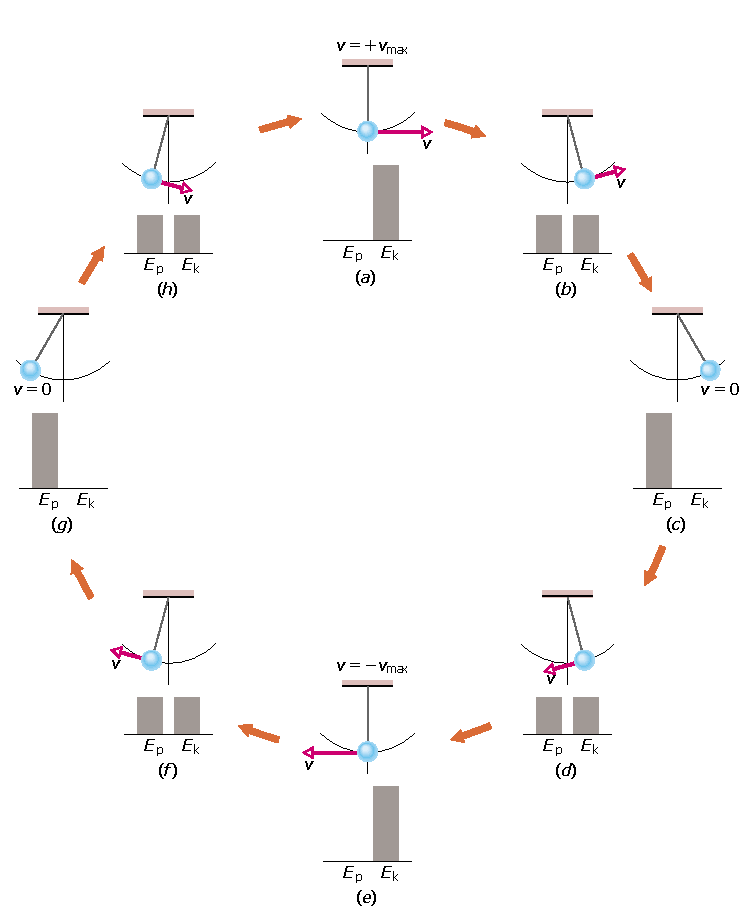
\includegraphics[width=0.9\linewidth]{fyz_fig029.pdf}
      \caption{ (Kyvadlo, jehož hmotnost je soustředěna v kuličce upevněné na konci vlákna, koná 
                 kmitavý pohyb. Obrázek zachycuje jednu periodu tohoto pohybu. Během periody se 
                 hodnoty kinetické i potenciální energie soustavy kyvadlo + Země spojitě mění, ale 
                 její celková mechanická energie zůstává zachována. Pro názornost můžeme použít i 
                 takovou představu, že se celková energie \(E\) spojitě „přelévá“ z jedné formy v 
                 druhou (potenciální v kinetickou a naopak). Ve stavech (a) a (e) je celková  
                 energie dána pouze energií kinetickou. Kulička je v nejnižším bodě a má největší 
                 rychlost. Ve stavech (c) a (g) je naopak celková energie rovna energii 
                 potenciální, neboť kulička je v nejvyšším bodě a její rychlost je v tom okamžiku  
                 nulová. V případech (b), (d), (f) a (h) tvoří jak kinetická, tak potenciální    
                 energie právě polovinu energie celkové. Pokud by se při kmitech kyvadla 
                 uplatňovaly třecí síly v závěsu nebo odporová síla vzduchu, energie \(E\) by se 
                 nezachovávala a kyvadlo by se nakonec zastavilo.\cite[s.~177]{Halliday2001})}
      \label{fyz:fig029}
    \end{figure}
    
  \section{Práce vykonaná gravitací}
    Další problém, jímž se budeme zabývat, je mnohem těžší. Týká se případu, kdy síly nejsou stálé 
    a svislé, jako byly předtím. Budeme například zkoumat pohyb planety kolem Slunce nebo družice 
    kolem Země.
    
    Nejdříve vezmeme v úvahu pohyb tělesa, které je v nějakém počátečním bodě \(1\) a řekněme, že 
    padá \emph{přímo} na Slunce nebo na Zemi (obr. \ref{fyz:fig024}). Bude za těchto okolností 
    platit zákon zachování energie? Jediný rozdíl proti předcházejícímu případu je ten, že nyní 
    není síla konstantní, ale mění se podél dráhy\footnote{ve správném názvosloví se v uvedeném 
    smyslu nepoužívá termín dráha, ale trajektorie (pod dráhou se rozumí délka trajektorie).}. Jak 
    víme, síla je rovna součinu \(\kappa\frac{M}{r^2}\) a hmotnosti \(m\) pohybujícího se tělesa. 
    Samozřejmě, když těleso padá na Zemi, narůstá se zvětšující se dráhou jeho kinetická energie, 
    právě tak jako v případě, kdy jsme změnu síly s výškou neuvažovali. Je otázkou, zda lze najít 
    jiné vyjádření pro potenciální energii (odlišné od \(mgh\)), takovou funkci vzdálenosti od 
    Země, že zákon zachování energie bude stále splněn.
    
    \luagraphic[0.9]{fyz_fig024.pdf}{Těleso o malé hmotnosti \(m\) padá pod vlivem gravitace na 
    těleso o velké hmotností \(M\) (\cite[s.~188]{Feynman01})}{fyz:fig024}

    Tento jednorozměrný případ lze snadno zvládnout, neboť víme, že změna kinetické energie je 
    rovna integrálu od jednoho konce dráhy k druhému z  \(-\kappa\frac{Mm}{r^2}\) vynásobeného 
    změnou polohy \(\dd{r}\)
    \begin{equation}\label{fyz:eq038}
      T_2 - T_1 = -\int_{1}^{2}\kappa\,M\,m\frac{\dd{r}}{r^2}.
    \end{equation}
    tomto případě nevystupuje ve vztahu žádný kosinus, neboť síla i změna polohy mají stejný směr. 
    Integrál z \(\frac{dr}{r^2}\) není těžké vypočítat, je roven \(-\frac{1}{r}\), takže
    \begin{equation}\label{fyz:eq039}
      T_2 - T_1 = +\kappa\,M\,m\left(\dfrac{1}{r_2} - \dfrac{1}{r_1}\right).
    \end{equation}
    Tak jsme dostali nové vyjádření pro potenciální energii. Vztah (\ref{fyz:eq039}) říká, že 
    veličina \(\frac{1}{2}mv^2 - \kappa\frac{Mm}{r}\) vypočítaná v bodě \(1\) nebo \(2\) nebo v 
    kterémkoli jiném místě, má konstantní hodnotu.
    
    Nyní máme vztah pro výpočet potenciální energie při vertikálním pohybu v gravitačním poli. 
    Objevuje se zajímavý problém. Lze v gravitačním poli dosáhnout \emph{věčného pohybu}? 
    Gravitační pole se mění, na různých místech má různý směr a různou sílu. Lze najít pevnou dráhu 
    bez tření, po níž bychom těleso zvedli z nějakého bodu do jiného bodu, pak ho přenesli po 
    oblouku do dalšího bodu, spustili ho o určitou vzdálenost, dále jím pohnuli pod určitým sklonem 
    nějakým jiným směrem atd. tak, aby po návratu do výchozího bodu vykonala gravitační síla 
    určitou práci a kinetická energie tělesa se zvětšila? Lze vyznačit takovou dráhu, po níž se 
    těleso po návratu bude pohybovat o něco rychleji než předtím, takže vytvoří věčný pohyb? 
    Protože perpetuum mobile není možné, mělo by jít dokázat, že ani toto není možné. Měli bychom 
    dokázat tvrzení: Neexistuje-li tření, těleso by se nemělo vrátit ani větší ani menší rychlostí 
    - mělo by být schopné pohybovat se jen dokola po této uzavřené dráze. Vyjádřeno jinak: 
    \emph{Celková práce vykonaná gravitačními silami po dráze celého cyklu, musí být rovna nule}, 
    neboť kdyby nebyla rovna nule, bylo by možné takovýmto kruhovým pohybem získávat energii. 
    (Ukáže-li se, že tato práce je menší než nula, že by se tedy po proběhnutí jednoho cyklu 
    rychlost zmenšila, stačí, abychom prostě změnili směr pohybu na opačný, neboť síly závisí jen 
    na poloze, ne na směru pohybu. Bude-li v jednom směru práce kladná, v opačném směru záporná, 
    tedy půjdeme-li tím či oním směrem, bude nenulová hodnota znamenat věčný pohyb.)
    
    Skutečně je tato práce rovna nule? Pokusme se ukázat, že ano. Nejprve více či méně objasníme, 
    proč je rovna nule a pak to trochu podrobněji prozkoumáme matematicky. Předpokládejme, že 
    použijeme jednoduchou dráhu, jako je dráha na obr, \ref{fyz:fig025}, kde se malé těleso 
    pohybuje z bodu \(1\) do bodu \(2\), pak po oblouku do bodu \(3\), dále do bodu \(4\), potom do 
    bodů \(5\), \(6\), \(7\), \(8\)  a nakonec zpět do bodu \(1\). Všechny úseky dráhy jsou buď 
    radiální nebo jsou to oblouky kružnic se středem v hmotnosti \(M\), Jaká práce se vykoná při 
    pohybu tělesa podél této dráhy? Mezi body \(1\) a \(2\) je to \(\kappa Mm\) vynásobeno rozdílem 
    \(\frac{1}{r}\) mezi těmito body
    \begin{equation*}
      W_{12} = \int_{1}^{2}\vec{F}\cdot\dd{\vec{s}} = 
             - \int_{1}^{2}\kappa Mm\frac{\dd{r}}{r^2}
             = \kappa\,M\,m\left(\dfrac{1}{r_2} - \dfrac{1}{r_1}\right).
    \end{equation*} 
    Z bodu \(2\) do bodu \(3\) svírá síla s dráhou přesně pravé úhly, takže \(W_{23} = 0\). Práce z 
    bodu \(3\) do bodu \(4\) je
    \begin{equation*}
      W_{34} = \int_{3}^{2}\vec{F}\cdot\dd{\vec{s}}
             = \kappa\,M\,m\left(\dfrac{1}{r_4} - \dfrac{1}{r_3}\right).
    \end{equation*} 
    Podobně \(W_{45} = 0\), \(W_{56} = \kappa Mm\left(\dfrac{1}{r_6} - \dfrac{1}{r_5}\right)\),
    \(W_{67}=0\), \(W_{78} = \kappa Mm\left(\dfrac{1}{r_8} - \dfrac{1}{r_7}\right)\). Tedy
    \begin{equation*}
      W = \kappa\,M\,m\left(-\dfrac{1}{r_1} + \dfrac{1}{r_2} 
                            -\dfrac{1}{r_3} + \dfrac{1}{r_4}
                            -\dfrac{1}{r_5} + \dfrac{1}{r_6}
                            -\dfrac{1}{r_7} + \dfrac{1}{r_8}\right).
    \end{equation*} 
    Všimněme si však, že \(r_2 = r_3, r_4 = r_5, r_6 = r_7, r_8 = r_1\). Proto \(W = 0\)
    
    \begin{figure}[ht!]  %\ref{fyz:fig025}
      \centering
      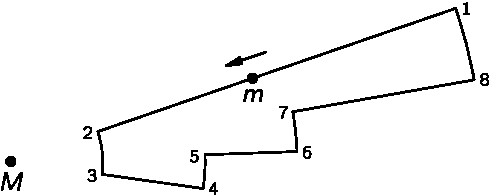
\includegraphics[width=0.8\linewidth]{fyz_fig025.pdf}
      \caption{Uzavřená dráha v gravitačním poli (\cite[s.~190]{Feynman01})}
      \label{fyz:fig025}
    \end{figure}
    Samozřejmě bychom mohli namítnout, zda to není příliš jednoduchá křivka. Co se stane, 
    použijeme-li nějakou reálnou křivku? Zkusme to s takovouto křivkou. Především bychom rádi 
    poznamenali, že jakoukoli křivku lze dostatečně dobře napodobit pomocí sledu pilových zubů 
    (obr. \ref{fyz:fig025}), a tak bychom mohli naše tvrzení dokázat, avšak bez určité analýzy není 
    ihned jasné, že práce vykonaná při pohybu podél trojúhelníka, ač malého, je rovna nule. 
    Zvětšíme jeden z trojúhelníků, jako na obr. \ref{fyz:fig026}. Je práce vykonaná při přechodu po 
    obvodu trojúhelníka z \(A\) do \(B\) a do \(C\) rovna práci vykonané při přímém přechodu z 
    \(A\) do \(C\)? Předpokládejme, že síla působí v určitém směru. Vyberme si například takový 
    trojúhelník, jehož strana \(BC\) leží v tomto směru. Předpokládáme, že trojúhelník je tak malý, 
    že síla po celém trojúhelníku je v podstatě, konstantní. Jaká práce se vykoná při přechodu z 
    \(A\) do \(C\)? Je to
    \begin{equation*}
      W_{AC} = \int_A^C\vec{F}\cdot\dd{\vec{s}} = FS\cos\vartheta,
    \end{equation*} 
    neboť síla je konstantní. Nyní vypočítejme, jaká práce se vykoná při přechodu podél dalších 
    dvou stran trojúhelníka. Na vertikální straně \(AB\) je síla kolmá k \(\dd{s}\), takže zde je 
    práce rovna nule. Na horizontální straně \(BC\) je
    \begin{equation}\label{fyz:eq044}
      W_{BC} = \int_B^C\vec{F}\cdot\dd{\vec{s}} = Fx.
    \end{equation} 

    Vidíme, že práce, která se koná při přechodu po odvěsnách malého trojúhelníka je rovna práci 
    při přechodu po přeponě, neboť \(s\cos\vartheta\) je rovno \(x\). Předtím jsme si ukázali, že 
    výsledek je roven nule pro jakoukoli dráhu složenou z řady malých schodů, jako na obr. 
    \ref{fyz:fig025}, a nyní vidíme, že vykonáme stejnou práci, když si cestu zkrátíme napříč, 
    místo toho, abychom šli po schůdcích (pokud jsou to schůdky dostatečně jemné a na takové je 
    vždy můžeme upravit), proto \textbf{práce vykonaná podél jakékoli uzavřené dráhy v gravitačním 
    poli je rovna nule}.
    
    To je velmi pozoruhodný výsledek. Říká o planetárním pohybu něco, co jsme předtím nevěděli. 
    Tvrdí, že jestliže se planeta pohybuje kolem Slunce (aniž by nablízku byla jiná tělesa, tj. za 
    nepřítomnosti jiných sil), pohybuje se takovým způsobem, že když od druhé mocniny rychlosti v 
    kterémkoli bodě dráhy odečteme nějaké konstanty vydělené průvodičem \(r\) v tomto bodě, 
    dostaneme pro každý bod oběžné dráhy stejnou hodnotu. Například, čím blíže ke Slunci je 
    planeta, tím rychleji se pohybuje. O kolik rychleji? O takovouto hodnotu: Kdybychom při pohybu 
    kolem Slunce změnili směr její rychlosti (nikoli však velikost této rychlosti) tak, aby se 
    planeta pohybovala radiálně a nechali bychom ji spadnout z určité vzdálenosti až na požadovanou 
    délku průvodiče, její nová rychlost by byla taková, jakou má planeta na této oběžné dráze, 
    protože jde jen o jiný případ komplikované dráhy. Kdyby se planeta vrátila do původní 
    vzdálenosti, její kinetická energie by byla stejná jako předtím. Ať už planeta doletí do 
    nějakého bodu po nenarušené dráze nebo směr jejího pohybu byl změněn prostřednictvím vazeb bez 
    tření, její kinetická energie v tomto bodě bude stejná.

    \begin{figure}[ht!]  %\ref{fyz:fig026}
      \centering
      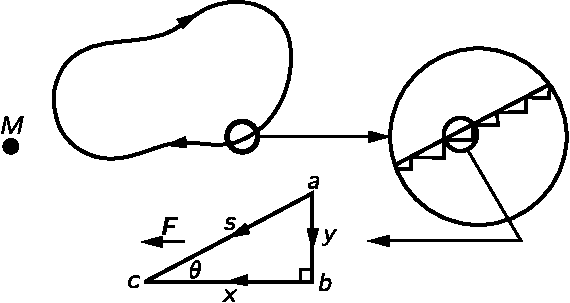
\includegraphics[width=0.7\linewidth]{fyz_fig026.pdf}
      \caption{„Hladká“ uzavřená dráha: zvětšenina části dráhy aproximované posloupností radiálních 
      a obvodových kroků a pohled na jeden zvětšený schod (\cite[s.~191]{Feynman01})}
      \label{fyz:fig026}
    \end{figure}
    Proto, když provádíme numerickou analýzu pohybu planety po oběžné dráze, jak jsme již dělali, 
    můžeme se krok za krokem přesvědčit výpočtem energie, zda jsme neudělali chybu. Energie by se 
    neměla měnit. Pro oběžnou dráhu podle tab. \ref{fyz:tab001} se však energie\footnote{v 
    jednotkách \ref{fyz:tab001} je energie rovna \(\frac{1}{2}(v_x^2+v_y^2)-\frac{1}{r}\).} mění 
    podél dráhy přibližně o \num{1.5}\%. Proč? Buď proto, že jsme při numerické metodě použili 
    konečné intervaly, nebo proto, že jsme udělali chybu někde v aritmetice.
    
    Sledujme, co se děje s energií v jiném případě - v případě tělesa zavěšeného na pružině. 
    Vychýlíme-li těleso z jeho rovnovážné polohy, je síla, která ho chce vrátit zpět, úměrná 
    velikosti výchylky. Lze najít zákon zachování energie při těchto podmínkách? Ano, neboť práce 
    vykonaná takovouto silou je rovna
    \begin{equation}\label{fyz:eq045}
      W = \int_0^x\vec{F}\cdot\dd{\vec{x}} = \int_0^x(-kx)\dd{x} = -\frac{1}{2}kx^2,
    \end{equation}
    tedy pro těleso na pružině platí, že součet kinetické energie oscilujícího tělesa a 
    \(\frac{1}{2}kx^2\) je roven konstantě. Podívejme se, jak to probíhá. Těleso potáhneme směrem 
    dolů; je v klidu, takže jeho rychlost je rovna nule. Ale \(x\) není rovno nule, je maximální, 
    je tu tedy nějaká energie, zřejmě potenciální. Když uvolníme těleso, nastane kmitání, které 
    nebudeme podrobně rozebírat. \emph{V každém okamžiku však musí být součet kinetické a 
    potenciální energie konstantní.} Například, když těleso prochází rovnovážným bodem, je rovno 
    nule, tehdy je \(v^2\) největší. Čím je větší \(x^2\), tím je menší \(v^2\) atd., takže při 
    kmitání se udržuje rovnováha mezi \(x^2\)a \(v^2\). Tak jsme dostali další pravidlo: Je-li síla 
    rovna \(-kx\), je potenciální energie pružiny rovna \(\frac{1}{2}kx^2\).
    
  \section{Sčítání energií}
    Nyní přejdeme k obecnějším úvahám o tom, co se stane, máme-li velké množství těles. 
    Předpokládejme, že máme komplikovaný problém mnoha těles, označených indexy \(i= 1, 2, 3, 
    \ldots\). Jež na sebe všechna gravitačně působí. Co se bude dít? Dokážeme, že když sečteme 
    kinetické energie všech částic a k tomu přičteme součet z jejich vzájemné gravitační 
    potenciální energie \(-\kappa\frac{Mm}{r_{ij}}\), vypočtenou přes všechny páry částic, 
    dostaneme tento celkový součet rovnající se konstantě
    \begin{equation}\label{fyz:eq024}
      \frac{1}{2}\sum_im_iv_i^2 + 
      \sum_{\substack{\text{páry } ij}}\left(\frac{\kappa\,m_i\,m_j}{r_{ij}}\right)= \text{konst.}
    \end{equation}
    
    Jak to dokážeme? Budeme diferencovat obě strany podle času a přesvědčíme se, že dostaneme nulu. 
    Diferencováním \(\frac{1}{2}m_iv_i^2\) dojdeme k derivacím rychlostí, což jsou vlastně síly, 
    jako v rovnici (\ref{fyz:eq027}). Za tyto síly dosadíme jejich vyjádření známé z 
    \emph{Newtonova gravitačního zákona} a všimneme si, že to, co zůstane, je právě časová derivace 
    výrazu
    \begin{equation*}
      \frac{1}{2}\sum_im_iv_i^2 + 
      \sum_{\substack{\text{páry } ij}}\left(-\frac{\kappa\,m_im_j}{r_{ij}}\right).
    \end{equation*}
    Derivace kinetické energie podle času je
    \begin{align}
      \der{ }{t}\sum_{\substack{i}}\frac{1}{2}m_iv_i^2 &=
                \sum_{\substack{i}}m_i\vec{v}_i\cdot\left(\der{\vec{v}_i}{t}\right)  
              = \sum_{\substack{i}}\vec{F}_i\cdot\vec{v}_i                           \nonumber \\
             &= \sum_{\substack{i}}\left(\sum_{\substack{i}}
               -\frac{\kappa\,m_i\,m_j\vec{r}_{ij}}{r_{ij}^3}\right)\cdot\vec{v}_i.  
                \label{fyz:eq040}
    \end{align}
    Derivace potenciální energie podle času je
    \begin{equation}\label{fyz:eq041}
      \der{ }{t}\sum_{\substack{\text{páry}} ij}\left(-\frac{\kappa\,m_i\,m_j}{r_{ij}}\right) =
                \sum_{\substack{\text{páry}}}\left(+\frac{\kappa\,m_i\,m_j}{r_{ij}}\right)
                     \left(\der{r_{ij}}{t}\right).
    \end{equation}
    Ale
    \begin{equation}\label{fyz:eq042}
      r_{ij} = \sqrt{(x_i - x_j)^2 + (y_i - y_j)^2 + (z_i - z_j)^2},
    \end{equation}
    a tedy
    \begin{align*}
      \der{r_{ij}}{t} 
        &= \frac{1}{2r_{ij}}
        \Big[\Big.
           (x_i - x_j)\left(\der{x_i}{t} - \der{x_j}{t}\right) +   \\ 
        &+ (y_i - y_j)\left(\der{y_i}{t} - \der{y_j}{t}\right) +   \\
        &+ (z_i - z_j)\left(\der{z_i}{t} - \der{z_j}{t}\right)    
        \Big.\Big]                                                 \\
        &= \vec{r}_{ij}\cdot\frac{v_i - v_j}{r_{ij}} 
         = \vec{r}_{ij}\cdot\frac{v_i}{r_{ij}} + \vec{r}_{ji}\cdot\frac{v_j}{r_{ji}},
    \end{align*}
    protože \(\vec{r}_{ij} = - \vec{r}_{ji}\) zatímco \(r_{ij} = r_{ji}\).
    
    Tedy pro sumu \(\der{ }{t}\sum_{\substack{\text{páry}}}
    \left(-\frac{\kappa\,m_i\,m_j}{r_{ij}}\right)\) dostaneme
    \begin{equation}\label{fyz:eq043}
    %  \der{ }{t}\sum_{\substack{\text{páry}}}\left(-\frac{\kappa\,m_i\,m_j}{r_{ij}}\right) =
     =  \sum_{\substack{\text{páry}}}
              \left[
                \frac{\kappa\,m_i\,m_j\vec{r}_{ij}}{r_{ij}^3}\cdot\vec{v}_i +
                \frac{\kappa\,m_i\,m_j\vec{r}_{ji}}{r_{ji}^3}\cdot\vec{v}_j 
              \right].
    \end{equation}
    Nyní si musíme pozorně všimnout, co znamenají symboly \(\sum_i\left(\sum_j\right)\) a 
    \(\sum_{\substack{\text{páry}}}\). V rovnici \ref{fyz:eq041} \(\sum_i\left(\sum_j\right)\) 
    znamená, že \(i\) nabývá postupně všech hodnot \(i = 1, 2, 3 \ldots\) a pro každou hodnotu 
    \(i\) nabývá index \(j\) všech hodnot kromě \(i\). Takže je-li \(i = 3\), pak \(j\) nabývá 
    hodnot \(1, 2, 4, \ldots\)
    
    Na druhé straně symbol \(\sum_{\substack{\text{páry}}}\)  v rovnici (\ref{fyz:eq043}) znamená, 
    že daná dvojice \(i\) a \(j\) se v sumě vyskytuje jen jednou, takže pár částic \num{1} a 
    \num{3} přispívá do sumy jen jedním členem. V souladu s tím můžeme připustit, aby index \(i\) 
    nabýval postupně všech hodnot \(1, 2, 3, \ldots\) a pro každé \(i\) nechť \(j\) nabývá jen 
    hodnot větších než \(i\). Tedy jestliže \(i = 3\), \(j\) může nabývat hodnot \(4, 5, 6, 
    \ldots\). Všimněme si však, že pro každou hodnotu indexů \(i\), \(j\) se v sumě nacházejí 
    příspěvky od dvou členů, v jednom je \(v_i\) a v druhém je \(v_j\), a že tyto členy jsou 
    podobné členům ve vztahu  (\ref{fyz:eq041}), kde jsou v sumě zahrnuty všechny hodnoty \(i\) a 
    \(j\) (kromě \(i=j\)). Proto, porovnáme-li příslušné výrazy člen po členu, vidíme, že rovnice  
    (\ref{fyz:eq043}) a  (\ref{fyz:eq041}) jsou si přesně rovny, pouze mají opačné znaménko, takže 
    derivace podle času ze součtu kinetické a potenciální energie je skutečně rovna nule. Z toho 
    vyplývá, že pro systém mnoha těles je \emph{kinetická energie dána součtem příspěvků od 
    jednotlivých těles a potenciální energie je také dána prostě součtem potenciálních energií 
    všech párů}. Proč zde vystupuje energie každého páru, můžeme pochopit takto: Předpokládejme, že 
    chceme vypočítat celkovou práci, kterou je třeba vynaložit, abychom tělesa dostali na určité 
    vzdálenosti od sebe. Toho můžeme dosáhnout pomocí více kroků tím, že je po jednom přeneseme z 
    nekonečna, kde na sebe silově nepůsobí. Nejprve přeneseme první těleso, k čemuž není potřeba 
    žádné práce, neboť nejsou přítomna žádná tělesa, která by na něho mohla silově působit Dále 
    přeneseme druhé těleso, což si vyžádá určitou práci, jmenovitě \(W_{1,2} = - 
    \frac{\kappa\,m_1\,m_2}{r_{12}}\). Nyní, a to je důležité, předpokládejme, že přeneseme další 
    těleso do třetí polohy. Síla, která působí na třetí těleso je v každém okamžiku rovna součtu 
    dvou sil - sil vyvolaných prvním a druhým tělesem. Proto \emph{vykonaná práce je rovna součtu 
    prací vykonaných každou silou zvlášť} neboť lze-li \(\vec{F}_3\) rozložit na součet dvou sil
    \begin{align*}
     \vec{F}_3 &= \vec{F}_{13} + \vec{F}_{23},        \\
      \shortintertext{pak práce je rovna}
      \int\vec{F}_3\cdot\dd{\vec{s}} 
                &=  \int\vec{F}_{13}\cdot\dd{\vec{s}} + 
                    \int\vec{F}_{23}\cdot\dd{\vec{s}}
                 = W_{13} + W_{23}. 
    \end{align*}
    Znamená to, že vykonaná práce je rovna součtu prací vykonaných proti první a druhé síle, jako 
    by každá síla působila nezávisle. Pokračujeme-li takovýmto způsobem dále, vidíme, že celková 
    práce potřebná k vytvoření dané konfigurace těles, je přesné rovna hodnotě, uvedené ve vztahu 
    (\ref{fyz:eq024}) jako potenciální energie. Potenciální energii můžeme psát ve tvaru součtu 
    přes všechny dvojice částic, neboť pro gravitaci platí \textbf{princip superpozice sil}.
    
   
  \section{Gravitační pole velkých těles}
    Nyní vypočítáme pole, s nimiž se ve fyzice setkáváme za takových okolností, které souvisejí s 
    \emph{rozložením hmoty}. Dosud jsme brali v úvahu jen částice a neuvažovali jsme o rozložení 
    hmoty, ale je zajímavé provést i výpočet sil způsobených ne jen jednou, ale více částicemi. 
    Nejprve vypočteme gravitační sílu způsobenou nekonečnou hmotnou rovinou. Síla způsobená touto 
    hmotnou plochou působící na jednotkovou hmotnost v daném bodě \(P\) (obr. \ref{fyz:fig027}), 
    bude samozřejmě směřovat k ploše. Nechť je vzdálenost bodu od roviny \(a\) a na jednotkovou 
    plochu této roviny připadá hmotnost \(\mu\). Budeme předpokládat, že \(\mu\) je konstanta, tj. 
    že jde o homogenní vrstvu materiálu. Jak velké pole \(\dd{\vec{K}}\) vytvoří hmotnost 
    \(\dd{m}\), jež se nachází ve vzdálenosti mezi \(\varrho\) a \(\varrho +d\varrho\) od bodu 
    \(0\), jenž je nejbližším bodem roviny k bodu \(P\)? Bude to pole \(\dd{K} = 
    \kappa(d\,m\frac{\vec{r}}{r^3})\). Toto pole má směr \(r\), ale víme, že když sečteme malé 
    vektory \(\dd{\vec{K}}\), abychom dostali \(\vec{K}\), zůstane z něho jen \(x\)-ová složka. 
    Zřejmě \(x\)-ová složka \(\dd{\vec{K}}\) je rovna
    \begin{equation}\label{fyz:eq046}
      \dd{K_x} = \kappa\frac{d\,mr_x}{r^3} = \kappa\frac{d\,ma}{r^3}.
    \end{equation}
    Všechny hmotnosti \(dm\), jež jsou stejné vzdáleny od bodu \(P\), dávají stejné \(dK_x\), proto 
    hned můžeme místo \(dm\) psát celkovou hmotnost prstence mezi \(\varrho +d\varrho\), tj. 
    \(dm=\mu2\pi\varrho\,d\varrho\) ( \(2\pi\varrho\,d\varrho\) je plocha prstence s poloměrem 
    \(\varrho\) šířkou \(d\varrho\), jestliže platí \(d\varrho \ll \varrho\)). To znamená, že
    \begin{equation}\label{fyz:eq047}
      \dd{K_x} = \kappa\mu2\pi\varrho\frac{d\,\varrho a}{r^3}.
    \end{equation}
    Ale \(\varrho\,d\,\varrho = r\,d\,r\) neboť \(r^2 = \varrho^2 + a^2\). Proto
    \begin{equation}\label{fyz:eq048}
      K_x = 2\pi\kappa\mu\,a\int_a^\infty\frac{d\,r}{r^2}
          = 2\pi\kappa\mu\,a\left(\frac{1}{a} - \frac{1}{\infty}\right) = 2\pi\kappa\mu.
    \end{equation}

    \begin{figure}[ht!]  %\ref{fyz:fig027}
      \centering
      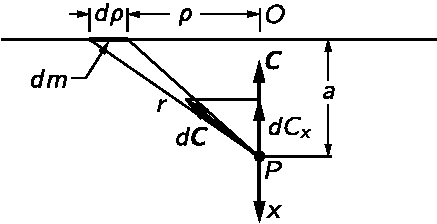
\includegraphics[width=0.7\linewidth]{fyz_fig027.pdf}
      \caption{Gravitační síla způsobí \(\vec{F}\) na hmotný bod vyvolaná hmotností nekonečné 
               rovinné desky (\cite[s.~195]{Feynman01})}
      \label{fyz:fig027}
    \end{figure}
    Síla nezávisí na \(a\)! Proč? Nezmýlili jsme se? Zdálo by se, že čím je vzdálenost větší, tím 
    je síla slabší. Nikoli! Při malé vzdálenosti se přitažlivost většiny hmoty projevuje pod 
    nepříznivým úhlem a při velké vzdálenosti má větší část hmoty příznivější polohu k tomu, aby 
    způsobovala přitažlivost směrem k rovině. Při jakékoli vzdálenosti leží hmota, která se nejvíce 
    uplatňuje, v určitém kuželi. Se vzrůstající vzdáleností se síla zmenšuje nepřímo úměrně druhé 
    mocnině vzdálenosti, ale v tomtéž kuželi, pod stejným úhlem, bude \emph{mnohem víc} hmoty, 
    úměrné druhé mocnině vzdálenosti! Tuto analýzu lze provést přesně, stačí, když si všimneme, že 
    diferenciální příspěvek v kterémkoli daném kuželi skutečně nezávisí na vzdálenosti, neboť s 
    měnící se vzdáleností se velikost síly dané hmoty a množství hmoty v kuželi mění recipročně. 
    Samozřejmě, síla ve skutečnosti není konstantní, neboť na druhé straně roviny má opačné 
    znaménko.
    
   Tak jsme v podstatě vyřešili i problém z elektřiny: máme-li elektricky nabitou desku s nábojem 
    \(\sigma\) na jednotku plochy, pak je elektrické pole v daném bodě mimo desku rovno 
    \(\frac{\sigma}{2\varepsilon_0}\) a směřuje od desky, jestliže je tato nabita kladně, a k ní, 
    je-li nabita záporně. K důkazu nám stačí, všimneme-li si, že \(\kappa\) má v gravitaci stejnou 
    úlohu jako \(\frac{1}{4\pi\varepsilon_0}\) v elektrostatice.
    
    Předpokládejme nyní, že máme dvě desky; jednu s kladnou hustotou náboje \(+\sigma\) a druhou se 
    zápornou hustotou náboje \(-\sigma\) ve vzdálenosti \(D\) od první. Jaké je jejich pole? Z 
    vnější strany desek je rovno nule. Proč? Protože jedna deska přitahuje a druhá odpuzuje. 
    \emph{Síla nezávisí} na vzdálenosti, proto se jejich účinky ruší! Mezi deskami je síla dvakrát 
    větší než síla jedné desky, tj. \(E = \frac{\sigma}{\varepsilon_0}\) a směřuje od kladné k 
    záporné desce.
    
    Nyní se dostáváme k nejzajímavějšímu a nejdůležitějšímu problému, jehož řešení jsme celou dobu 
    předpokládali. Síla, kterou Země působí na hmotný bod na svém povrchu nebo mimo něj, je taková, 
    jako kdyby \emph{hmotnost celé Země byla soustředěna v jejím středu}. Platnost tohoto 
    předpokladu není zřejmá, neboť těsně u zemského povrchu je část hmotnosti velmi blízko, část je 
    dále atd. Zdá se být div, že po sečtení všech těchto sil by výsledná síla měla být stejná jako 
    ta, kterou bychom dostali, kdybychom hmotnost celé Země stlačili do jejího středu!
    
    \begin{figure}[ht!]  %\ref{fyz:fig028}
      \centering
      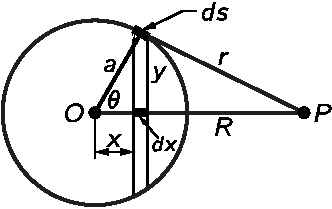
\includegraphics[width=0.6\linewidth]{fyz_fig028.pdf}
      \caption{Tenká sférická slupka hmoty nebo náboje (\cite[s.~195]{Feynman01})}
      \label{fyz:fig028}
    \end{figure}
    Dokážeme správnost tohoto zázraku. Za tím účelem nahraďme představu celé Země tenkou homogenní 
    kulovou slupkou. Nechť \(m\) je její celková hmotnost. Vypočtěme potenciální energii části o 
    hmotnosti \(m'\) ve vzdálenosti \(R\) od středu koule (obr. \ref{fyz:fig028}) a objasníme si, 
    že potenciální energie je stejná, jako kdyby hmotnost \(m\) byla soustředěna v jednom bodě ve 
    středu koule. (S potenciální energií se nám pracuje snadněji než s intenzitou pole, neboť 
    nemusíme brát v úvahu úhly, prostě sečteme potenciální energie všech částí hmotnosti.) 
    Označíme-li vzdálenost určitého rovinného řezu od středu \(x\), pak celá hmotnost ve vrstvě 
    \(dx\) má stejnou vzdálenost \(r\) od \(P\) a potenciální energie vyvolaná tímto kulovým pásem 
    je \(-\frac{\kappa\,m'dm}{r}\). Jakou hmotnost má vrstva \(dx\)? Je rovna
    \begin{equation}\label{fyz:eq049}
      dm = 2\pi\,y\mu ds = \frac{2\pi y\mu dx}{\sin\vartheta} 
         = \frac{2\pi y\mu dxa}{y} = 2\pi a\mu dx.
    \end{equation}
    kde \(\mu = \frac{m}{4\pi a^2}\) je plošná hustota hmotnosti kulové slupky. (Je obecným 
    pravidlem, že povrch kulového pásu je úměrný jeho výšce). Proto potenciální energie způsobená 
    hmotností dm je rovna
    \begin{equation}\label{fyz:eq050}
      dU = -\frac{\kappa\,m'\,dm}{r} = -\frac{\kappa\,m'\,2\pi a\mu dx}{r}.
    \end{equation}
    Vidíme však, že
    \begin{align*}
      r^2  &= y^2 + (R-x)^2 = y^2 + x^2 R^2 - 2Rx = a^2 + R^2 - 2Rx,           \\
      \shortintertext{tedy}
      2rdr &= -2Rdx \quad \text{neboli} \quad \frac{dx}{r} = - \frac{dr}{R}. \\
      \shortintertext{proto}
      dU   &= - \frac{\kappa\,m'2\pi a\mu dr}{R},
    \end{align*}
    a tak
    \begin{equation}
      U  =   \frac{\kappa\,m'2\pi a\mu}{R}\int_{R-a}^{R+a}dr              
         = - \frac{\kappa\,m'2\pi a\mu}{R}2a                                
         = - \frac{\kappa m'(4\pi a^2\mu)}{R} = -\frac{\kappa m'\,m}{R}.    \label{fyz:eq051}
    \end{equation}    
    Pro tenkou kulovou slupku tedy má hmotnost \(m'\) takovou potenciální energii, jako kdyby 
    hmotnost slupky byla zkoncentrována v jejím středu. Zemi si můžeme představit rozdělenou na 
    celou řadu sférických slupek, jejichž příspěvky k potenciální energii závisí jen na jejich 
    hmotnostech a na vzdálenosti od středu. Když je sečteme, dostaneme \emph{celkovou hmotnost}. 
    Proto působí Země tak, jakoby celá její hmotnost byla v jejím středu!
    
    Všimněme si, co se stane, bude-li bod P uvnitř slupky. Provedeme-li stejný výpočet pro \(P\) 
    uvnitř, opět dostaneme rozdíl dvou \(r\), ale nyní ve formě \((a + R) - (a - R) =2R\), tj. 
    dvojnásobek vzdálenosti od středu, jinými slovy, potenciální energie je rovna \(U = - 
    \frac{\kappa m'\,m}{a}\), což je \emph{nezávislé} na \(R\) a na poloze, tj. \emph{kdekoli} 
    uvnitř bude energie stejná. Proto k pohybu uvnitř není potřebná síla, ani se nekoná práce. 
    Je-li potenciální energie stejná, bez ohledu na to, kde se v kulové slupce těleso nachází, 
    nemůže na něj působit žádná síla. Uvnitř tedy síla nepůsobí, jen mimo kouli, a tato síla je 
    taková, jakoby celá hmotnost kulové slupky byla soustředěna v jejím středu.

  \section{Práce}
    Při studiu kteréhokoli technického předmětu, k jehož pochopení je důležitá matematika, stojíme 
    před úlohou porozumět a zapamatovat si množství fakt a myšlenek. Ty jsou navzájem spjaty 
    určitými vztahy, jejichž existenci lze \uv{dokázat} nebo \uv{ukázat}. Snadno se splete důkaz se 
    vztahem, který ustanovuje. Samozřejmě, co je důležité naučit se a zapamatovat si, to je samotný 
    vztah a ne jeho důkaz. Pak v jakékoli situaci můžeme buď říci \uv{lze ukázat, že to a to je 
    pravda}, nebo to můžeme ukázat sami. Použitý důkaz je téměř ve všech případech tak přizpůsoben, 
    aby se především dal snadno provést na tabuli nebo na papíře, a aby byl i co možná 
    nejuhlazenější. Důkaz se v důsledku toho může omylem zdát jednoduchým, zatímco ve skutečnosti 
    mohl autor zkoušet vypočítat tutéž věc různými způsoby a možná na něm pracoval celé hodiny, než 
    našel nejvhodnější cestu - tu, která vede k výsledku za nejkratší dobu! Když před sebou máme 
    důkaz, je důležité uvědomit si ne samotný důkaz, ale fakt, že to a to lze dokázat. Samozřejmě, 
    jestliže důkaz obsahuje nějaký nový matematický postup nebo \uv{trik}, který jsme ještě 
    neznali, je třeba mu věnovat pozornost - ne však samotnému triku, ale použité matematické 
    myšlence.

    První myšlenka, s níž bude třeba si trochu pohrát, je ta, že \textbf{síla koná práci}. 
    Fyzikální význam slova \emph{práce} se liší od běžného významu tohoto slova. Fyzikální práci 
    lze vyjádřit ve tvaru \(\int\vec{F}\cdot\dd{\vec{s}}\), což je \emph{křivkový integrál} ze 
    skalárního součinu \(\vec{F}\) a \(\dd{s}\). To například znamená, že působí-li síla na objekt 
    v jednom směru a objekt sám se posune v jiném směru, pak práci koná jen \emph{složka síly ve 
    směru posunutí}. Kdyby byla například síla konstantní a posunutí by bylo jen o malou vzdálenost 
    \(\Delta s\), pak by práce vykonaná konstantní silou na této dráze byla rovna jen složce síly 
    podél \(\Delta s\) vynásobené \(\Delta s\). Pravidlo zní „síla krát dráha“, ale myslíme tím jen 
    složku síly ve směru posunutí krát \(\Delta s\) nebo složku posunutí ve směru síly krát 
    \(F\), což je \emph{ekvivalentní}. Je jasné, že síla, která svírá s posunutím pravý úhel, 
    nekoná žádnou práci.
    
    Rozložíme-li vektor posunutí \(\Delta\vec{s}\) dále na složky, nebo jinými slovy, chceme-li se 
    na skutečné posunutí \(\Delta\vec{s}\) dívat jako na posunutí \(\Delta x\) ve směru osy \(x\), 
    \(\Delta y\) ve směru osy \(y\) a \(\Delta z\) ve směru osy \(z\), pak práci, která se koná 
    posunutím tělesa z jednoho místa na druhé, lze vypočítat ze tří částí: vypočtením práce 
    vykonané ve směru osy \(x\), ve směru osy \(y\) a ve směru osy \(z\). K určení práce 
    vykonané ve směru osy \(x\) je třeba znát složku síly ve směru osy \(x\), tj. \(F_x\) atd., 
    takže práce je rovna \(F_x\Delta x + F_y\Delta y + F_z\Delta z\). V případě, že síla není 
    konstantní a jde o komplikovaný křivočarý pohyb, musíme celou dráhu rozdělit na množství malých 
    posunutí \(\Delta s\), sečíst práci vykonanou pohybem tělesa podél všech \(\Delta s\) a určit 
    limitu pro \(\Delta s\) jdoucí k nule. To je význam pojmu \uv{\textbf{křivkový integrál}}.
    
    Vše, co jsme dosud řekli, je obsaženo ve vztahu \(W=\vec{F}\cdot\dd\vec{s}\). Můžeme říci, že 
    je to nádherný vztah, ale něco zcela jiného je pochopit ho i v jeho důsledcích.
    
    Ve fyzice má slovo práce tak odlišný význam od běžného smyslu, že je třeba si dobře uvědomit, 
    za jakých okolností se navzájem liší. Například, podle fyzikální definice práce, jestliže 
    chvíli držíme zvednuté padesátikilové závaží, nekonáme práci. Naproti tomu je jasné, že se 
    začneme potit, třást se a těžko dýchat, jako bychom běželi nahoru po schodech. Ale při běhu 
    nahoru po schodech se práce koná, při běhu dolů po schodech se podle fyziky práce získává, 
    zatímco držením tělesa v pevné poloze, se práce nekoná. Tedy fyzikální definice práce se liší 
    od fyziologické definice z důvodů, které stručně prozkoumáme.
    
    Zůstává faktem, že drží-li někdo závaží, koná „fyziologickou“ práci. Proč se potí? Proč se 
    potřebuje najíst, aby udržel závaží? Jaké procesy probíhají v jeho těle, které se namáhá na 
    plné obrátky, jen aby udrželo závaží? Vždyť závaží lze bez námahy udržet, když ho položíme na 
    stůl. Stůl ho tiše a pokojně udrží ve stejné výšce, aniž bychom museli nějak dodávat energii! 
    Fyziologie nám dává toto vysvětlení. Člověk i jiné druhy živočichů mají dva druhy svalů. Jsou 
    to \emph{příčně pruhované} nebo \emph{kosterní} svaly (například na rukách), které lze vědomě 
    ovládat a \emph{hladké svaly} (například svaly střev nebo velký sval měkkýšů, který zavírá 
    lasturu). Hladké svaly jsou pomalé, ale mohou se „zatnout“, což znamená, že jestliže chce 
    měkkýš zavřít lasturu v určité poloze, udrží ji v ní i proti značně velké síle, jež by mu v tom 
    chtěla zabránit. Navzdory zátěži si udrží danou polohu celé hodiny, aniž by se unavil, podobně 
    jako stůl, na kterém je závaží. Sval se zatne, jeho molekuly dočasně fixují svou polohu, nekoná 
    se práce a měkkýš nemusí vynakládat žádnou námahu. Skutečnost, že když chceme udržet závaží, 
    musíme vynaložit úsilí, souvisí s konstrukcí příčně pruhovaných svalů. Když svalové vlákno 
    dostane nervový impulz, na okamžik se stáhne a znovu se uvolní. Když něco držíme, do svalu 
    přichází obrovské množství nervových impulzů, tíha tělesa se vyrovnává stahy mnoha svalových 
    vláken, zatímco jiná vlákna odpočívají. Důkazem je fakt, že když držíme těžké závaží a unavíme 
    se, začnou se svaly třást. Třesou se proto, že přívaly nervových signálů nejsou pravidelné, 
    sval je unaven a nereaguje dostatečně rychle. Proč jsou svaly zkonstruovány tak neefektivně? To 
    přesně nevíme, ale v přírodě neexistují rychlé hladké svaly. K držení závaží by bylo možné 
    využít hladkých svalů efektivněji, protože by se prostě zatnuly. Práce by se nekonala a nebylo 
    by třeba energie. Tyto svaly mají však svou nevýhodu - jsou velmi pomalé.
    
    Ale vraťme se k fyzice a položme si otázku: Proč potřebujeme znát vykonanou práci? Je to i 
    zajímavé i užitečné, neboť \textbf{práce, kterou dodá částici výslednice všech sil, jež na ni 
    působí, se přesně rovná změně kinetické energie částice}. Znamená to, že jestliže na těleso 
    působí síla, a těleso nabírá rychlost, platí
    \begin{equation}\label{fyz:eq018}
      \Delta(v^2) = \frac{2}{m}\vec{F}\cdot\Delta\vec{s}.
    \end{equation}
  
  \section{Vázaný pohyb}
    Síly a práce mají ještě další zajímavou vlastnost. Mějme \emph{nakloněnou nebo zakřivenou 
    cestu} a částici, jež se bude po ní pohybovat bez tření. Nebo uvažujme kyvadlo - \emph{závaží 
    na vlákně}. Vlákno \emph{omezuje} pohyb závaží na pohyb po kružnici kolem bodu závěsu. Bod 
    závěsu lze změnit, necháme-li vlákno narazit na kolík. Pak se dráha závaží bude skládat ze dvou 
    kružnic s různými poloměry. To jsou příklady tzv. \textbf{tuhé vazby bez tření}
    
    Při pohybu s tuhou vazbou bez tření nekoná vazba žádnou práci, neboť síly vazby svírají s 
    dráhou pohybu pravý úhel. \textbf{Vazbovými silami rozumíme síly, jež působí na těleso pod 
    vlivem samotné vazby - reakce podložky nebo napětí vlákna.}
    
    Síly, které působí na pohyb částice pod vlivem gravitace po nakloněné dráze jsou dost složité. 
    Je tu síla vazby, gravitační síla atd. Když však při výpočtu pohybu vyjdeme ze \emph{zachování 
    energie} a jen samotné gravitační sily, dostaneme správný výsledek. Zdá se to být divné, neboť 
    to není ten správný postup - měli bychom počítat s \textbf{výslednicí sil}. Nicméně se ukáže, 
    že je to práce \emph{vykonaná} gravitační silou, která je rovna změně kinetické energie, 
    protože práce vykonaná vazbovou složkou síly je \emph{rovna} nule (obr. \ref{fyz:fig021}).
  
    \begin{figure}[ht!]  %\ref{fyz:fig021}
      \centering
      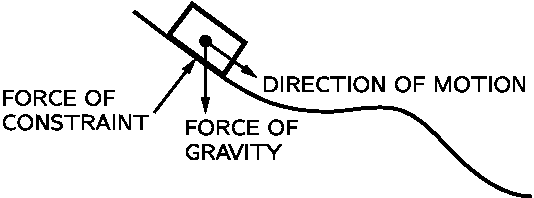
\includegraphics[width=0.7\linewidth]{fyz_fig021.pdf}
      \caption{Síly působící na těleso, které klouže bez tření (\cite[s.~201]{Feynman01})}
      \label{fyz:fig021}
    \end{figure}
    Důležitá je tu ta vlastnost, že lze-li sílu rozložit na součet dvou nebo více „částí“, pak 
    práce, vykonaná výslednou silou při pohybu po určité dráze je rovna součtu prací vykonaných 
    různými „složkami“ síly, na něž byla výsledná síla rozložena. Rozložíme-li sílu na vektorový 
    součet více sil (gravitační síly, vazbové síly atd. nebo \(x\)-ovou složku všech sil, 
    \(y\)-ovou složku všech sil nebo jakýmkoli jiným způsobem), pak se práce vykonávaná celkovou 
    silou rovná součtu prací vykonaných všemi složkami, na něž jsme celkovou sílu rozložili.
  
  \section{Konzervativní síly}
    V přírodě se vyskytují určité síly (například gravitační síla), které se vyznačují velmi 
    pozoruhodnou vlastností - \emph{jsou konzervativní} (nejde o žádné politické ideje, je to jen 
    jeden z těch \uv{šílených} názvů).  Vypočítáme-li práci vykonanou silou při přemístění tělesa z 
    jednoho bodu do druhého podél nějaké zakřivené dráhy, \emph{závisí} tato práce obecně na 
    \emph{dráze}, ale ve zvláštních případech na ní nezávisí. \textbf{Nezávisí-li práce na dráze, 
    říkáme, že síla je konzervativní}. Jinak řečeno, jestliže se integrál síly vynásobené 
    přírůstkem vzdálenosti při přechodu z bodu \(1\) do bodu \(2\) na obr. \ref{fyz:fig020} spočítá 
    nejprve podél křivky \emph{A} a pak podél křivky \emph{B}, jestliže přitom dostaneme stejné 
    množství joulů, jestliže dále toto platí pro \emph{každou dráhu}, na níž leží body \(1\) a 
    \(2\), a jestliže toto tvrzení platí \emph{nezávisle na tom, které dva body bereme v úvahu}, 
    pak říkáme, že síla je konzervativní. Za takových okolností lze \emph{integrál práce} mezi body 
    \(1\) a \(2\) vypočítat jednoduchým způsobem a můžeme uvést výsledný vzorec. Obecně to není tak 
    jednoduché, neboť musíme specifikovat i dráhu, ale v případě, že práce nezávisí na tvaru dráhy, 
    je samozřejmé, že závisí jen na polohách \(1\) a \(2\).
    
    \luagraphic[0.7]{fyz_fig020.pdf}{Možné dráhy mezi dvěma body v silovém poli 
    (\cite[s.~202]{Feynman01})}{fyz:fig020}

    Abychom dokázali platnost těchto závěrů, vezměme si pevný bod \(P\) v libovolné poloze (obr. 
    \ref{fyz:fig020}). Pak lze dráhový integrál práce z bodu \(1\) do bodu \(2\) vypočítat jako 
    práce vykonaná po dráze z bodu \(1\) do \(P\) plus práce po dráze z \(P\) do \(2\), neboť síly 
    jsou konzervativní a vykonaná práce nezávisí na tvaru dráhy. Práce, která se koná při pohybu z 
    bodu \(P\) do určitého bodu v prostoru, je funkcí polohy tohoto bodu. Samozřejmě, že závisí i 
    na bodu \(P\), ale v naší analýze ho považujeme za pevný. Za tohoto předpokladu práce, vykonaná 
    při pohybu z bodu \(P\) do bodu \(2\), je funkcí konečné polohy bodu \(2\). Závisí na tom, kde 
    se bod \(2\) nachází; přemístíme-li těleso do nějakého jiného bodu, dostaneme jiný výsledek.

    Tuto funkci polohy budeme značit - \(U(x, y, z)\), a jestliže půjde o bod \(2\), jehož 
    souřadnice jsou \((x_2, y_2, z_2)\), budeme jako zkratku pro \(U(x_2, y_2, z_2)\) psát prostě 
    \(U(2)\). Práci, vykonanou při posunutí tělesa z bodu \(1\) do bodu \(P\), lze napsat jako 
    práci vykonanou při \emph{opačném posunutí}, přičemž je třeba změnit znaménka všech \(\dd{s}\). 
    To znamená, práce vykonaná při posunutí z bodu \(1\) do bodu \(P\) je rovna práci vykonané při 
    posunutí z bodu \(P\) do bodu \(1\) se \emph{znaménkem} \(-\)
    \begin{equation}\label{fyz:eq016}
      \int_1^P\vec{F}\cdot\dd{s} = \int_1^P\vec{F}\cdot(-\dd{s}) = \int_P^1\vec{F}\cdot\dd{s}
    \end{equation}
    Takže práce při posunutí z bodu \(P\) do bodu \(1\) je rovna \(-U(1)\) a z bodu \(P\) do bodu 
    \(2\) je rovna \(- U(2)\). Proto integrál od \(1\) do \(2\) je roven \(- U(2)\) plus \(- U(l)\) 
    zpětným směrem, tj. \(+ U(l) - U(2)\):
    \begin{align}
      U(1) &= - \int_P^1\vec{F}\cdot\dd{\vec{s}},  \nonumber\\
      U(2) &= - \int_P^2\vec{F}\cdot\dd{\vec{s}},  \nonumber\\
      \int_1^2\vec{F}\cdot\dd{\vec{s}} &= U(1) - U(2). \label{fyz:eq017}
    \end{align}
    Veličina \(U(l) - U(2)\) se nazývá změna potenciální energie a \(U\) nazýváme potenciální 
    energií. Říkáme, že těleso má potenciální energii \(U(2)\), jestliže se nachází v poloze \(2\) 
    a v poloze \(1\) má potenciální energii \(U(l)\). Nachází-li se v bodě \(P\), má nulovou 
    potenciální energii.
    
    Kdybychom místo bodu \(P\) použili kterýkoli jiný bod, řekněme bod \(Q\) vyšlo by, že 
    \emph{potenciální energie se mění jen o aditivní konstantu}. Protože zachování energie závisí 
    na \emph{změnách} energie, nic se nezmění, když k potenciální energii přičteme takovou 
    konstantu. Proto bod \(P\) je libovolný. Máme tedy dvě tvrzení:
    \begin{itemize}
      \item \textbf{Práce vykonaná silou je rovna změně kinetické energie.}
      \item Matematicky pro konzervativní sílu platí, že \textbf{vykonaná práce je rovna záporné   
            změně funkce \(U\) nazvané potenciální energií.}
    \end{itemize}
    Z těchto dvou tvrzení vyplývá, že \textbf{působí-li jen konzervativní síly, součet energie 
    \(U\) zůstává konstantní:}
    \begin{equation}\label{fyz:eq015}
      T + U = \text{konst}.
    \end{equation}
    Podívejme se na vztahy pro výpočet potenciální energie v několika konkrétních případech. V 
    případě homogenního gravitačního pole, nebudeme-li se pohybovat ve výškách srovnatelných s 
    poloměrem Země, je síla stálá a směřuje vertikálně. Vykonaná práce je prostě rovna síle
    vynásobené vzdáleností. Tedy
    \begin{equation}\label{fyz:eq019}
      U(z) = mgz.
    \end{equation}
    a bod \(P\), jenž odpovídá \emph{nulové} potenciální energii, bude kdekoli v rovině \(z=0\). 
    Kdybychom chtěli, můžeme říci, že potenciální energie bude například \(mg(z - 6)\) a všechny 
    výsledky našeho rozboru by zůstaly stejné, jen hodnota potenciální energie pro \(z=0\) by byla 
    \(- 6 mg\)\footnote{Samozřejmě s fyzikálním rozměrem energie.}. Na tom však nezáleží, neboť v 
    úvahu se berou jen změny potenciální energie.
    
    Energie potřebná k stlačení lineární pružiny o vzdálenost \(x\)  z rovnovážné polohy je rovna
    \begin{equation}\label{fyz:eq020}
      U(x) = \frac{1}{2}kx^2
    \end{equation}
     a potenciální energie je rovna nule v bodě \(x = 0\), tj. v rovnovážné poloze. Znovu bychom 
     mohli přidat libovolnou konstantu.
    
    Gravitační potenciální energie pro bodové hmotnosti \(M\) a \(m\) vzdálené od sebe na 
    vzdálenost \(r\) je rovna
    \begin{equation}\label{fyz:eq021}
      U(r) = - \kappa\frac{Mm}{r}. 
    \end{equation}
    V tomto případě byla konstanta zvolena tak, aby se potenciál \emph{ztratil v nekonečnu}. Stejný 
    vztah samozřejmě platí i pro elektrické náboje, neboť pro ně platí stejný zákon.
    \begin{equation}\label{fyz:eq022}
      U(r) = - \frac{1}{4\pi\varepsilon_0}\frac{q_1q_2}{r}. 
    \end{equation}
    Vezměme si nyní jeden z těchto vztahů, abychom se přesvědčili, zda mu rozumíme.
    
    \emph{Otázka}: Jakou rychlost musí mít raketa, aby se odpoutala od Země?
    
    \emph{Řešení}: Součet kinetické a potenciální energie musí být konstantní. Odpoutat se znamená 
    vzdálit se na milióny kilometrů. Má-li raketa dostatek energie k odpoutání se, můžeme 
    předpokládat, že v takové vzdálenosti bude její rychlost rovna nule, raketa bude téměř stát. 
    Nechť \(a\) je \emph{poloměr Země} a \(M\) je její hmotnost. Součet kinetické a potenciální 
    energie je na začátku roven \(\frac{1}{2}mv^2 - \kappa\frac{Mm}{a}\) a musí být roven celkové 
    energii na konci pohybu. Kinetickou energii na konci pohybu budeme považovat za nulovou, neboť 
    raketa by se měla vzdalovat již v podstatě s nulovou rychlostí a potenciální energie je rovna 
    \(\kappa Mm\) děleno nekonečnem, což je nula. Takže na jedné straně rovnice je nula, z čehož 
    vyplývá, že druhá mocnina rychlosti musí být rovna \(2\kappa\frac{M}{a}\) . Ale 
    \(2\kappa\frac{M}{a^2}\) je veličina, kterou nazýváme \textbf{gravitačním zrychlením} \(g\). 
    Takže
    \begin{equation}\label{fyz:eq023}
      v^2 = 2ga. 
    \end{equation}
    
    Jakou rychlostí se musí pohybovat družice, aby stále obíhala kolem Země? To jsme již dříve 
    vypočítali a zjistili jsme, že \(v^2=\kappa\frac{M}{a}\). K odpoutání se od Země tedy potřebuje 
    rychlost rovnou \(\sqrt{2}\) násobku rychlosti, kterou potřebujeme k tomu, abychom právě 
    obíhali kolem Země u jejího povrchu. K odpoutání se od Země tedy potřebujeme dvakrát tolik 
    energie (neboť energie závisí na druhé mocnině rychlosti) než k jejímu oblétnutí. Proto 
    historicky prvním krokem bylo dostat družici na oběžnou dráhu kolem Země, k čemuž je potřebná 
    rychlost kolem \SI{7.8}{\km\per\s}. Druhým krokem bylo vyslat kosmickou loď tak, aby se nikdy 
    nevrátila na Zemi; k tomu bylo třeba dvakrát tolik energie neboli rychlost kolem 
    \SI{11.2}{\km\per\s}.
    
    V naší další diskuzi o potenciální energii uvažujme interakci dvou molekul nebo atomů, 
    například dvou atomů kyslíku. Když jsou od sebe velmi vzdálené, síla je přitažlivá a mění se 
    jako převrácená hodnota sedmé mocniny vzdálenosti, a když jsou velmi blízko, interakce je silně 
    odpudivá. Integrováním minus sedmé mocniny vzdálenosti (abychom našli potřebnou práci) 
    zjistíme, že potenciální energie \(U\), jež je funkcí vzájemné vzdálenosti dvou kyslíkových 
    atomů, se při velkých vzdálenostech mění jako minus šestá mocnina vzdálenosti.
    
    Jestliže nakreslíme závislost potenciální energie \(U(r)\) (obr. \ref{fyz:fig022}), pro velké 
    hodnoty \(r\) se chová jako \(r^{-6}\), když se však dostatečně přiblížíme, dostaneme se do 
    bodu \(d\), kde je minimum potenciální energie. Minimum potenciální energie pro \(r=d\) 
    znamená, že vychýlíme-li se z bodu \(d\) o malou vzdálenost, vykonaná práce, která je rovna 
    změně potenciální energie při této výchylce, je přibližně rovna nule, neboť v minimu křivky se 
    potenciální energie mění jen velmi málo. V tomto bodě nepůsobí síla, což znamená, že je 
    rovnovážným bodem. Jiný způsob jak je možné se přesvědčit, zda je to bod rovnovážný, je ten, že 
    k vychýlení z bodu \(d\) kterýmkoli směrem je potřebná energie. Když se dva atomy kyslíku 
    ustálí v poloze, kde již silou, jež je mezi nimi, nelze uvolnit více energie, nacházejí se v 
    nejnižším energetickém stavu a jejich vzdálenost bude \(d\). Takto vypadá kyslíková molekula za 
    studená. Když ji zahřejeme, atomy se rozkmitají a vzdálí se, až je můžeme zcela oddělit. 
    Potřebujeme k tomu určitou práci či energii, jež je rovna rozdílu potenciálních energií mezi 
    \(r = d\) a \(r=\infty\). Pokusíme-li se atomy k sobě velmi těsně přiblížit, energie prudce 
    vzrůstá, neboť se navzájem odpuzují.    
    
    \begin{figure}[ht!]  %\ref{fyz:fig022}
      \centering
      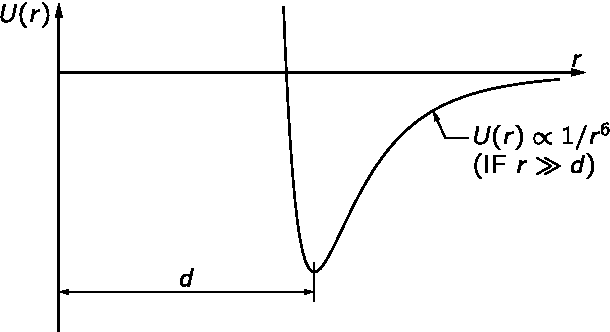
\includegraphics[width=0.8\linewidth]{fyz_fig022.pdf}
      \caption{Potenciální energie mezi dvěma atomy jako funkce jejich vzájemné vzdálenosti 
               (\cite[s.~202]{Feynman01})}
      \label{fyz:fig022}
    \end{figure}
    Tyto věci připomínáme proto, že koncepce síly není zvlášť vhodná pro kvantovou mechaniku, kde 
    je přirozenější koncepce energie. Zatímco pojmy síly a rychlosti se „vytratí“ při studiu 
    složitějších sil v jádře, mezi molekulami apod., \emph{koncepce energie zůstává}. Proto v 
    učebnicích kvantové mechaniky najdeme grafy potenciální energie, ale velmi zřídka, jestliže 
    vůbec někdy, najdeme grafické znázornění síly působící mezi dvěma molekulami, neboť lidé, kteří 
    studují tyto jevy, myslí spíše v pojmech energie než síly.
    
    Dále si všimněme, že jestliže na těleso působí více konzervativních sil současně, je 
    \textbf{potenciální energie tělesa rovna součtu potenciálních energií od každé síly zvlášť}. Je 
    to stejné tvrzení, jako jsme měli předtím, neboť dá-li se síla vyjádřit jako vektorový součet 
    více sil, pak práce vykonaná výslednou silou je rovna součtu prací vykonaných jednotlivými 
    silami a lze ji vyjádřit jako změny potenciální energie odděleně pro každou sílu. Takže 
    \emph{celková potenciální energie je rovna součtu jednotlivých příspěvků}.
    
    Lze provést zobecnění i pro systém navzájem interagujících těles, jako jsou Jupiter, Saturn, 
    Uran atd. nebo kyslíku, dusíku, uhlíku atd., jež navzájem interagují v párech prostřednictvím 
    sil, které jsou všechny konzervativní. V takovém případě je kinetická energie celé soustavy 
    prostě rovna součtu kinetických energií všech atomů, planet nebo čehokoli a potenciální energie 
    soustavy je rovna součtu potenciálních energií vzájemných interakcí každého páru samostatně, 
    jakoby tam další ani nebyly. (To ve skutečnosti přesně neplatí pro molekulární síly a vztah je 
    o něco komplikovanější; určitě to však platí pro newtonovskou gravitaci a pro molekulární síly 
    je vztah vhodný jen přibližně. V případě molekulárních sil je možné hovořit o potenciální 
    energii, ale ta je o něco složitější funkcí poloh atomů než prostý součet příspěvků od párů.) 
    Proto speciálně v případě gravitace je potenciální energie rovna součtu ze \(- \kappa 
    \frac{m_im_j}{r_{ij}}.\) pro všechny páry \(i\) a \(j\), jak jsme ukázali ve vztahu 
    (\ref{fyz:eq024}). Rovnice (\ref{fyz:eq024}) je matematickým vyjádřením tvrzení, že součet 
    celkové kinetické energie a celkové potenciální energie se s časem nemění. Vypočítáme-li 
    celkovou kinetickou a potenciální energii planet, i když jakkoli obíhají, točí se a vrtí, 
    zjistíme, že tento součet zůstává konstantní.
    
  \section{Nekonzervativní síly}
    Dost času jsme se věnovali diskuzi o konzervativních silách, ale jak je to se silami, které 
    nejsou konzervativní? V této kapitole zaujmeme hlubší stanovisko než je obvyklé a řekneme, že 
    nekonzervativní síly neexistují! Skutečně, všechny základní síly v přírodě jsou konzervativní. 
    Není to důsledkem Newtonových zákonů. Co se týče samotného Newtona, věděl, že síly mohou být i 
    nekonzervativní, jako například tření, jež se zdá být nekonzervativním. Když říkáme, že se zdá, 
    přijímáme moderní názor, podle něhož bylo zjištěno, že všechny základní síly, síly interakcí 
    mezi částicemi na nejfundamentálnější úrovni, jsou konzervativní.
    
    Kdybychom například provedli analýzu systému, jako je kulová hvězdokupa (jejíž obrázek jsme již 
    viděli), v níž jsou tisíce interagujících hvězd, dostali bychom vzorec pro celkovou potenciální 
    energii jako prostý součet jednotlivých členů, přičemž se sčítá přes všechny hvězdné páry a 
    kinetická energie je rovna součtu kinetických energií všech jednotlivých hvězd. Hvězdokupa se 
    však pohybuje v prostoru i jako celek, a kdybychom od ní byli dostatečně vzdáleni, že bychom 
    neviděli detaily, mohli bychom si myslet, že je to jeden objekt. Kdybychom na ni nechali 
    působit síly, některé by ji poháněly jako celek a střed hvězdokupy by se pohyboval. Na druhé 
    straně se může stát, že část sil by se „vyplýtvala“ na zvětšení kinetické a potenciální energie 
    těles, která jsou uvnitř. Předpokládejme například, že působením těchto sil celá hvězdokupa 
    expanduje a že hvězdy se budou pohybovat rychleji. Celková energie systému se skutečně 
    zachovává, ale při pohledu zvenku našima nedokonalýma očima, kterýma nepostřehneme složitost 
    pohybu uvnitř, a uvažujíce kinetickou energii celého objektu jako by to byla energie jednoho 
    tělesa, by se nám zdálo, že energie se nezachovává, ale je to jen následek toho, že jsme 
    nepostřehli všechny detaily. Ukazuje se, že věci se mají takto: při detailním pohledu je 
    celková energie tohoto vesmírného objektu, kinetická plus potenciální, rovna konstantě.
    
    Při studiu látek v těch nejjednodušších detailech na úrovni atomů není vždy snadné rozdělit 
    celkovou energii na dvě složky - kinetickou a potenciální a takové rozdělení není vždy nutné. 
    Lze to však provést \emph{téměř} vždy, a proto můžeme říci, že to je možné a že součet 
    potenciální a kinetické energie světa je konstantní. Takže celkový součet potenciální a 
    kinetické energie v celém světě je konstantní a je-li „světem“ kousek izolovaného materiálu, 
    energie je konstantní, nepůsobí-li vnější síly. Jak jsme však dokázali, část kinetické energie 
    a potenciální energie objektu může být vnitřní energií, například energie vnitřních 
    molekulových pohybů, vnitřních v tom smyslu, že je nevidíme. Víme, že v poháru vody všechno 
    kmitá, všechny části se stále pohybují, uvnitř je tedy určitá kinetická energie, jíž si obvykle 
    ani nevšimneme. Pohyb atomů, jenž se projevuje jako teplo, nevidíme, proto ho nenazýváme 
    kinetickou energií, ale teplo je v první řadě kinetickou energií. Vnitřní potenciální energie 
    může existovat například ve formě chemické energie: spalováním benzínu se uvolňuje energie, 
    neboť potenciální energie atomů v jejich novém uspořádání je nižší, než byla původně. Přesněji, 
    teplo není jen čistou kinetickou energií, ale částečně i potenciální energií a obrácené tvrzení 
    platí o chemické energii, takže obě formy energie spojujeme dohromady a říkáme, že celková 
    kinetická a potenciální energie uvnitř objektu existuje z části ve formě tepla, z části ve 
    formě chemické energie a tak dále. Jinak ovšem všechny tyto formy energie považujeme za 
    „ztracenou“ energii, v uvedeném smyslu; ujasníme si to při studiu termodynamiky.
    
    Dalším příkladem bude tření. Není pravda, že kinetická energie se ztrácí za přítomnosti tření, 
    i když se smýkající těleso zastaví a zdá se, že kinetická energie se ztratila. Kinetická 
    energie se samozřejmě neztratila, neboť atomy uvnitř kmitají s větší kinetickou energií než 
    předtím a ačkoli to nevidíme, můžeme to zjistit měřením teploty. Samozřejmě, nevezmeme-li v 
    úvahu tepelnou energii, pak věta o zachování energie se bude jevit neplatnou.
    
    Jiný příklad, při němž se zdá, že zachování energie neplatí, vzniká, když se zajímáme jen o 
    část systému. Je zcela přirozené, že věta o zachování energie se bude zdát neplatnou, 
    zanedbáme-li tu část interakce, jež probíhá s nějakým vnějším objektem.
    
    V klasické fyzice se do potenciální energie zahrnuje jen gravitace a elektřina, ale dnes známe 
    jadernou energii i jiné druhy energie. Například světlo by v klasické teorii představovalo 
    novou formu energie, ale chceme-li, můžeme si představit, že světelná energie je kinetická 
    energie fotonu, takže náš vztah (\ref{fyz:eq015}) bude stále platit.
    
  \section{Potenciály a pole}
    Nyní rozebereme některé myšlenky spojené s potenciální energií a s koncepcí \textbf{pole}. 
    Předpokládejme, že máme dvě velká tělesa \(A\), \(B\) a třetí velmi malé těleso, na které 
    působí gravitační přitažlivost prvních dvou těles s výslednou silou \(\vec{F}\). Již v kapitole 
    \ref{fyz:IchapXII} jsme si všimli, že gravitační sílu, působící na částice, lze napsat 
    jako součin její hmotnosti \(m\) a vektoru \(\vec{K}\) který závisí jen na poloze 
    částice \cite[s.~204]{Feynman01}:
    \begin{equation}\label{fyz:eq001}
      \vec{F} = m \vec{K}
    \end{equation}
    
    Gravitaci lze tedy analyzovat,jestliže si představíme, že v každém bodě prostoru je dán vektor 
    \(\vec{K}\), jenž „působí“ na těleso, které tam můžeme vložit, ale který tam je sám, ať už tam 
    těleso, na které působí, vložíme nebo ne. Vektor \(\vec{K}\) má tři složky, z nichž každá je 
    funkcí \((x, y, z)\), tj. \emph{funkcí polohy v prostoru}. Takovouto veličinu nazýváme 
    \emph{polem} a říkáme, že tělesa \(A\) a \(B\) vytvářejí pole, tj. \uv{dělají} vektor 
    \(\vec{K}\). Vložíme-li těleso do pole, je síla, která na něho působí, rovna součinu jeho 
    hmotnosti a hodnoty vektoru pole v bodě, kde se těleso nachází.
    
    Totéž je možné provést s \textbf{potenciální energií}. Potenciální energii - integrál z výrazu 
    \((\text{\textbf{síla}})\cdot(\dd{\vec{s}})\) - můžeme napsat jako \(m\) krát integrál z 
    \((\text{\textbf{pole}})\cdot(\dd{\vec{s}})\), čímž se změní jen škála, takže potenciální 
    energii \(U(x, y, z)\) tělesa v bodě prostoru \((x, y, z)\) lze napsat jako \(m\) krát jiná 
    funkce, kterou můžeme nazvat \emph{potenciálem} \(\Psi\). Integrál \(\int\vec{K}\cdot\dd{s}= 
    -\Psi\) podobně jako \(\int\vec{F}\cdot\dd{s}= -U\) liší se navzájem škálovým faktorem:
    \begin{equation}\label{fyz:eq002}
      U = -\int\vec{F}\dd{\vec{s}} = -m\int\vec{K}\dd{\vec{s}} = m\Psi.
    \end{equation}
    Známe-li funkci \(\Psi(x, y, z)\), můžeme bezprostředně vypočítat potenciální energii tělesa v 
    každém bodě prostoru, jmenovitě \(U(x, y, z) = m\Psi(x, y, z)\), což se zdá být zcela triviální 
    záležitostí, ale ve skutečnosti to není triviální věc, protože někdy je mnohem výhodnější 
    popsat pole zadáním hodnoty \(\Psi\) celém prostoru než zadáním \(\vec{K}\). Místo tří 
    komplikovaných složek vektorové funkce je jednodušší zadat skalární funkci \(\Psi\). Navíc, 
    je-li pole vyvoláno více tělesy, mnohem snadněji lze vypočítat \(\Psi\) kteroukoli složku 
    \(\vec{K}\), neboť potenciály jsou skaláry a můžeme je tedy prostě sčítat, aniž bychom se 
    museli starat o směr. Dále, jak ihned uvidíme, pole \(\vec{K}\) lze snadno určit, známe-li 
    \(\Psi\).
    
    Předpokládejme, že v bodech \(1, 2 \ldots\) se nacházejí hmotné body o hmotnostech \(m_1, m_2, 
    \ldots\) a chceme znát potenciál \(\Psi\) v nějakém libovolném bodě \(P\). Je to prostě součet 
    potenciálů jednotlivých těles v bodě \(P\).
    \begin{equation}\label{fyz:eq003}
      \Psi(P) = \sum-\frac{\kappa m_i}{r_{ip}}, \quad i = 1, 2 \ldots
    \end{equation}
    
    Vztah, že potenciál je roven součtu potenciálů jednotlivých těles, jsme použili v předcházející 
    kapitole, k výpočtu potenciálu vytvořeného kulovou slupkou, sečtením příspěvků k 
    potenciálu v daném bodě od všech částí slupky. Výsledek výpočtu je graficky znázorněn na obr. 
    \ref{fyz:fig018}. Potenciál je záporný, pro \(r=\infty\) nabývá nulovou hodnotu, mění se jako 
    \(1/r\) pokud mění rovno \(a\) a uvnitř slupky je konstantní. Venku je potenciál roven 
    \(-\frac{\kappa\cdot m}{r}\), kde \(m\) je hmotnost slupky, což je stejný výsledek, jako kdyby 
    byla všechna látka soustředěna ve středu. To neplatí všude, uvnitř kulové slupky je potenciál 
    roven \(-\frac{\kappa\cdot m}{a}\) a je konstantní! \textbf{Kde je potenciál konstantní, tam 
    není pole}, je-li potenciální energie konstantní, neexistuje žádná síla, protože 
    přemisťujeme-li těleso z místa na místo v prostoru uvnitř slupky, je vykonaná práce přesně 
    rovna nule. Proč je tomu tak? Protože práce vykonaná při pohybu tělesa je rovna změně 
    potenciální energie vzaté záporně (nebo odpovídající integrál pole je roven změně potenciálu). 
    Ale potenciální energie je stejná v kterýchkoli dvou vnitřních bodech, takže změna potenciální 
    energie je rovna nule a při pohybu mezi dvěma vnitřními body se nekoná práce. Jediná možnost, 
    jak může být práce rovna nule při pohybu ve všech směrech, je ta, že nepůsobí vůbec žádná síla.
    
    \begin{figure}[ht!]  %\ref{fyz:fig018}
      \centering
      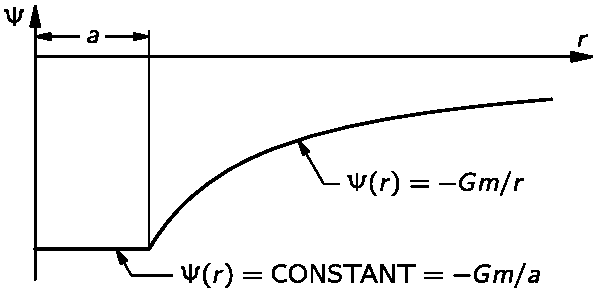
\includegraphics[width=0.8\linewidth]{fyz_fig018.pdf}
      \caption{Potenciál vyvolaný dutou koulí o poloměru \(a\) (\cite[s.~205]{Feynman01})}
      \label{fyz:fig018}
    \end{figure}    
    Zde můžeme najít klíč k řešení problému určení síly nebo pole, známe-li potenciální energii. 
    Předpokládejme, že známe potenciální energii tělesa, které je v bodě \((x, y, z)\) a chceme 
    vědět, jaká síla na něj působí. Jak uvidíme, se znalostí potenciálu v tomto jednom bodě problém 
    nevyřešíme. Potřebujeme znát hodnotu potenciálu i v okolních bodech. Proč? Jak lze vypočítat 
    složku síly \(x\)? (Dokážeme-li to, podobně najdeme i složku \(y\) a složku \(z\) a tím budeme 
    znát vlastně celou sílu.) Kdybychom tělesem pohnuli o malou vzdálenost \(\Delta x\), práce, 
    kterou vykoná síla, by byla rovna součinu \(x\)-ové složky síly a \(\Delta x\) (za předpokladu, 
    že \(\Delta x\) je dostatečně malé) a to by byla změna potenciální energie při přechodu z 
    jednoho bodu do druhého:
    \begin{equation}\label{fyz:eq004}
      \Delta W = - \Delta U = - F_x\Delta x.
    \end{equation}
    Pouze jsme zde využili vztah \(\int\vec{F}\cdot\dd{\vec{s}}\) pro \emph{velmi krátkou dráhu}. 
    Vydělením \(\Delta x\) dostáváme, že síla je rovna
    \begin{equation}\label{fyz:eq005}
      F_x = -\frac{\Delta U}{\Delta x}.
    \end{equation}
    
    Samozřejmě, tento výsledek není zcela přesný. Co chceme skutečně vypočítat, je limita 
    (\ref{fyz:eq005}) pro \(\Delta x\) stále menší a menší, protože výpočet platí \emph{přesně} 
    jen pro infinitezimální \(\Delta x\). Pak je to vlastně derivace \(U\) podle \(x\) a můžeme 
    psát \(-\der{U}{x}\). Ale \(U\) závisí na \(x, y, z\) a matematici vynalezli jiný symbol, jenž 
    nám má připomínat, že při diferencování takové funkce musíme být velmi opatrní a mít na paměti, 
    že uvažujeme jen změnu \(x\), zatímco \(y\) a \(z\) se nemění. Místo \(d\) píšou prostě 
    obrácenou šestku nebo \(\partial\). (V diferenciálním počtu se to mělo zavést již od začátku, 
    neboť \(d\) se chce člověku vykrátit, ale \(\partial\) ne!) Takže píšou \(\pder{U}{x}\) a 
    navíc, chtějí-li být mimořádně důslední a opatrní, napíšou vedle svislou čáru s malým \(yz\) 
    dole  \((\pder{U}{x})_{yz}\) což znamená: „Zderivuj \(U\) podle \(x\), zatímco \(y\) a \(z\) 
    nech konstantní.“ Znak toho, které proměnné se mají nechat konstantní, se obvykle vynechává, 
    neboť je to jasné z kontextu.Zato \emph{vždy} budeme psát \(\partial\) místo \(d\), aby bylo 
    jasné, že je to derivace, při níž některé další proměnné jsou konstantní. Nazývá se 
    \textbf{parciální derivací} a je to derivace v níž měníme jen část proměnných, v tomto případě 
    proměnnou \(x\).
    
    Máme tedy výsledek, že síla ve směru osy \(x\)je rovna záporně vzaté parciální derivaci \(U\) 
    podle \(x\)
    \begin{equation}\label{fyz:eq006}
      F_x = -\pder{U}{x}.
    \end{equation}
    Podobným způsobem diferencováním \(U\) podle \(y\) při konstantním \(x\) a \(z\) lze najít sílu 
    ve směru souřadnice \(y\). Třetí složka se vypočítá derivováním podle \(z\) při konstantním 
    \(x\) a \(y\):
    \begin{equation}\label{fyz:eq007}
      F_y = -\pder{U}{y}, \quad  F_z = -\pder{U}{z}.
    \end{equation}
    Tak lze vypočítat sílu z potenciální energie. Pole lze získat z potenciálu přesně stejným 
    způsobem
    \begin{equation}\label{fyz:eq008}
      K_x = - \pder{\Psi}{x},\quad K_y = - \pder{\Psi}{y},\quad K_z = - \pder{\Psi}{z}.
    \end{equation}
    Připomeňme ještě další označení, které zatím ještě nějakou dobu nebudeme potřebovat. Protože 
    \(\vec{K}\) je vektor se složkami \(x, y, z\) a získáváme ho pomocí symbolů \(\pder{ }{x}\), 
    \(\pder{ }{y}\) a \(\pder{ }{z}\) připomínají tyto symboly složky vektoru. Matematici vynalezli 
    nový symbol \(\nabla\), zvaný \uv{grad} nebo „gradient“, jenž není veličinou, ale je to 
    \textbf{operátor}, který ze \emph{skaláru udělá vektor}. Má tyto „složky“: složka \(x\) je 
    \(\pder{ }{x}\), složka \(y\) je \(\pder{ }{y}\), složka \(z\) je \(\pder{ }{z}\), a proto s 
    potěšením můžeme přepsat naše vztahy v elegantním tvaru
    \begin{equation}\label{fyz:eq009}
      \vec{F} = -\nabla U, \quad  \vec{K} = -\nabla\Psi.
    \end{equation}
    Používáme-li zápis s \(\nabla\), ihned vidíme, zda máme před sebou vektorové rovnice nebo ne. 
    Ve skutečnosti (\ref{fyz:eq009}) znamená přesně totéž jako rovnice (\ref{fyz:eq006}) a 
    (\ref{fyz:eq007}). Je to jen způsob jejich zápisu a protože se nám vždy nechce psát tři 
    rovnice, píšeme místo nich prostě \(\nabla U\).
    
    Ještě jeden příklad polí a potenciálů z elektřiny. V tomto případě je síla působící na 
    stacionární náboj rovna součinu náboje a elektrického pole: \(\vec{F}= q\vec{E}\). (Obecně 
    \(x\)-ová složka síly má i část, jež závisí na magnetickém poli. Z rovnice (\ref{fyz:eq011}) 
    lze snadno ukázat, že \emph{síla}, jež působí na částici díky \emph{magnetickému poli}, svírá 
    vždy \emph{pravý} úhel s rychlostí částice i s magnetickým polem. Protože síla magnetického 
    pole působí na pohybující se náboj pod pravým úhlem k směru rychlosti, \textbf{magnetické pole} 
    v tomto případě \textbf{nekoná práci}. Při výpočtech kinetické energie v elektrickém a 
    magnetickém poli nemusíme brát v úvahu příspěvek od magnetického pole, neboť toto pole nemění 
    kinetickou energii nebo vykonanou práci jako při gravitaci a můžeme vypočítat veličinu 
    \(\varphi\), jež je rovna \emph{zápornému dráhovému integrálu} z \(\vec{E}\cdot\dd{\vec{s}}\), 
    z libovolného pevného bodu do bodu, v němž potenciál počítáme. \emph{Potenciální energie v 
    elektrickém poli je pak právě rovna součinu náboje \(q\) a potenciálu \(\varphi\)}
    \begin{equation}\label{fyz:eq012}
      \varphi(r) = -\int\vec{E}\cdot\dd{\vec{s}}, \quad U = q\varphi.
    \end{equation}
    
    \begin{figure}[ht!]  %\ref{fyz:fig019}
      \centering
      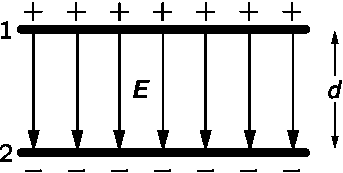
\includegraphics[width=0.6\linewidth]{fyz_fig019.pdf}
      \caption{Pole mezi rovnoběžnými deskami (\cite[s.~207]{Feynman01})}
      \label{fyz:fig019}
    \end{figure}   
    Vezměme jako příklad dvě paralelní kovové desky, každou s povrchovým nábojem \(\sigma\) na 
    jednotkové ploše, tzv. \textbf{rovinný kondenzátor}. Již dříve jsme vypočítali, že mimo 
    kondenzátor je síla nulová a že mezi deskami je konstantní elektrické pole ve směru od \(+\) k 
    \(-\) velikosti \(\frac{\sigma}{\varepsilon_0}\) (obr. \ref{fyz:fig019}). Chtěli bychom 
    zjistit, jaká práce se vykoná přenesením náboje z jedné desky na druhou. Práce bude rovna 
    integrálu z výrazu \((\text{\textbf{síla}})\cdot(\dd{\vec{s}})\), jenž lze napsat jako součin 
    náboje a potenciálu na první desce mínus tatáž veličina na druhé desce:
    \begin{equation}\label{fyz:eq013}
      W = \int_1^2\vec{F}\cdot\dd{\vec{s}} = q(\varphi_1 -\varphi_2).
    \end{equation}

    Tento integrál lze snadno vypočítat, neboť síla je konstantní a označíme-li vzdálenost desek 
    jako \(d\), dostáváme
    \begin{equation}\label{fyz:eq014}
      \int\vec{F}\cdot\dd{\vec{s}} = \frac{q\sigma}{\varepsilon_0}\int_1^2\dd{x} 
                                   = \frac{q\sigma d}{\varepsilon_0}.
    \end{equation}
    
    Rozdíl potenciálu \(\Delta\varphi = \dfrac{\sigma d}{\varepsilon_0}\) se nazývá \textbf{napětí} 
    a \(\varphi\) se měří ve \textbf{voltech}. Říkáme-li, že desky jsou nabité na určité napětí, 
    znamená to, že rozdíl potenciálů těchto desek je tolik a tolik voltů. Pro kondenzátor ze dvou 
    paralelních desek s plošnou hustotou náboje \(\pm\sigma\) je napětí nebo rozdíl potenciálů 
    desek roven \(\dfrac{\sigma d}{\varepsilon_0}\).
    
  \section{Přehled}
    \mbox{\textbf{Konzervativní síly}}: Síla působící na částici je \emph{konzervativní}, je-li 
    celková práce, kterou vykoná při pohybu částice po libovolné uzavřené trajektorii, nulová. 
    Ekvivalentní vyjádření: Síla působící na částici je konzervativní, jestliže práce, kterou 
    vykoná při přemístění částice mezi dvěma zadanými body, nezávisí na trajektorii, po které se
    částice pohybovala. Tíhová síla a pružná síla jsou konzervativní. Dynamická třecí síla je 
    \emph{nekonzervativní}.
    
  \section{Příklady a cvičení}  
    %-Dělová koule o hmotnosti $m = 24\,kg$ opustila hlaveň---------
    % !TeX spellcheck = cs_CZ
  \begin{example} Dělová koule o hmotnosti $m = 24\,kg$ opustila hlaveň rychlostí $v = 
    500\,ms^{-1}$ v čase $\tau=0.008\,s$ po zapálení roznětky. Jak velká síla na kouli působila, 
    jestliže předpokládáme rovnoměrně zrychlený pohyb koule v hlavni? Jak velká práce byla vykonána 
    na urychlení koule a jak dlouhá je hlaveň?\newline
    \textbf{Řešení:}
    \begin{itemize}
      \item Délka hlavně: $l=\frac{1}{2}at^2=\frac{1}{2}v\tau=\frac{1}{2}\cdot500\cdot0.008=2\,m$
      \item Síla působící na kouli: $F=m\frac{v}{\tau}=24\cdot\frac{500}{0.008}=1.5\times10^6\,N$
      \item Vykonaná práce při urychlování koule: $A=\frac{1}{2}mv^2=3\times10^6\,J$
    \end{itemize}
    \todo[inline]{exam004 dopočítat - pahýl}
 \end{example} 
    %---------------------------------------------------------------
%} %tikzset
%---------------------------------------------------------------------------------------------------